%!TEX root = tcc_final.tex
\chapter{Resultados}\label{chap5:resultados}
    Neste capítulo apresentaremos os testes executados para validar a implementação realizada neste trabalho. Para que seja possível termos um bom comparativo, realizamos os mesmos testes feitos por Jurak~\cite{Jurak2020COLREGS} em seu trabalho. Logo, testamos as alterações realizadas no sistema base para os encontros \textit{"Head On"}, \textit{"Overtaking"}, \textit{"Crossing from Left"} e \textit{"Crossing from Right"}. Com o intuito de evidenciar nossa implementação, realizamos um caso de teste adicional de \textit{"Crossing from Right"} onde a outra embarcação encontra-se parada e afastada o suficiente para que, quando executado com CPA, o sistema não considere uma situação de risco. Mesmo estando mais afastada, em um dado momento a outra embarcação é detectada pelo planejador local, fazendo com que ela seja considerada nas rotas locais planejadas a partir de então. Realizamos esse último caso de teste com e sem CPA. Para fins de análise apresentaremos as trajetórias realizadas pelas embarcações durante o teste, a distância entre elas, o tempo computacional necessário para planejar a rota local e \tcpa e o \dcpa calculados.
    
    Os testes foram realizados utilizando a ferramenta de simulação USV\_sim\footnote{\url{https://github.com/disaster-robotics-proalertas/usv_sim_lsa}}~\cite{Paravisi2018Toward}. Nela, utilizamos o barco de propulsão mostrado na Figura~\ref{fig:chap5_boat}. Os testes foram executados em um cenário virtual que simula o Arroio do Dilúvio, localizado em Porto Alegre - RS. Este cenário foi o mesmo utilizado por Jurak~\cite{Jurak2020COLREGS} em seu trabalho, que também apresenta a Figura~\ref{fig:chap5_diluvio}, ilustrando ambiente real (Figura~\ref{fig:chap5_diluvio_real}) e o ambiente simulado (Figura~\ref{fig:chap5_diluvio_simulado}).
    
    \begin{figure}[H]
		\centering
        \begin{subfigure}{0.4\textwidth}
            \centering
            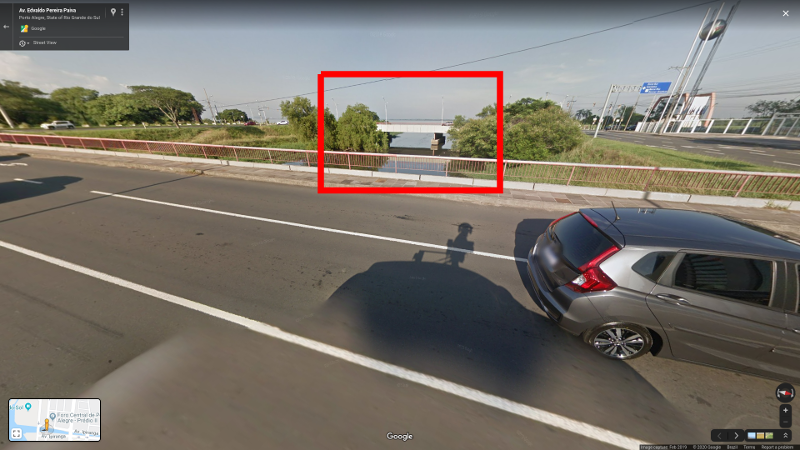
\includegraphics[width=\textwidth]{fig/chap5/diluvio_real.png}
            \caption{}
            \label{fig:chap5_diluvio_real}
        \end{subfigure}
        \begin{subfigure}{0.4\textwidth}
            \centering
            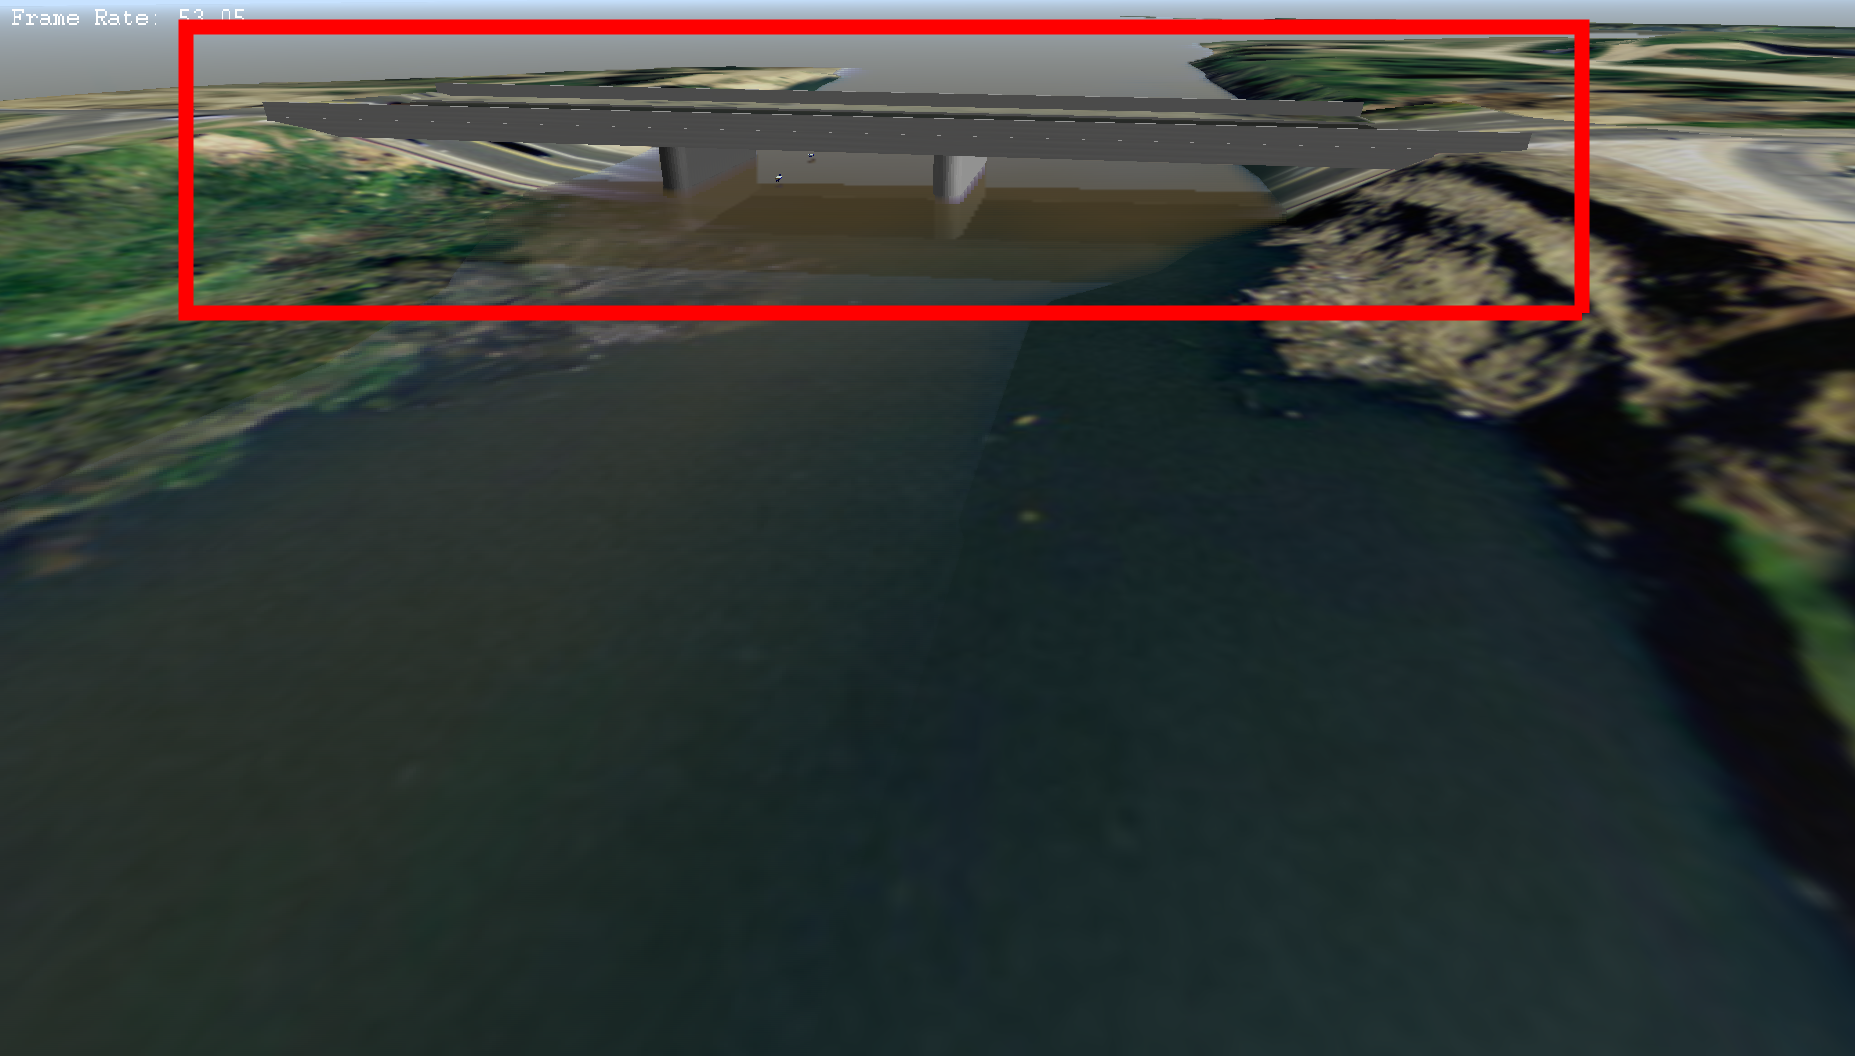
\includegraphics[width=\textwidth]{fig/chap5/diluvio_simulado.png}
            \caption{}
            \label{fig:chap5_diluvio_simulado}
        \end{subfigure}
    
    \caption{Ambiente real e ambiente simulado, apresentado por Jurak~\cite{Jurak2020COLREGS}}
    \label{fig:chap5_diluvio}
    \end{figure}
    % Comentário para evitar novo parágrafo
    \begin{figure}[H]
        \centering
        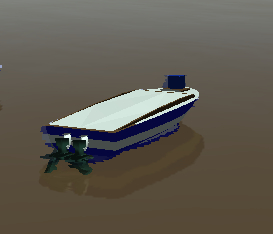
\includegraphics[scale=0.5]{fig/chap5/boat.jpg}
        \caption{Barco de propulsão utilizado nos testes.}
        \label{fig:chap5_boat}
    \end{figure}
    
    \section{Head On} \label{subchap5_headon}
        
        A Figura~\ref{fig:chap5_headon_paths} mostra a trajetória realizada pelas embarcações para o caso de teste \textit{"Head On"}, onde as embarcações vão uma de encontro a outra frente a frente. A linha azul representa o trajeto realizado pelo USV enquanto que a linha vermelha representa o trajeto realizado pela outra embarcação. Os pequenos triângulos, em cada uma das trajetórias no gráfico, indicam o sentido em que as embarcações se deslocaram e a posição em que cada uma das embarcações estava quando a distância entre elas foi a menor registrada durante todo o teste. A 
        distância, nesse caso, foi de 2,419m. A Figura~\ref{fig:chap5_headon_cpa} mostra as informações coletadas durante o teste a respeito do CPA. A Figura~\ref{fig:chap5_headon_tcpa} mostra graficamente, no tempo, o \tcpa calculado. O eixo horizontal representa unidades de tempo e o eixo vertical representa o \tcpa calculado na unidade de segundos, essas informações são válidas para todos os gráficos de \tcpa apresentados daqui para frente. Os vales gerados no gráficos indicam que a condição $\Vert\vec{v}_{A}-\vec{v}_{B}\Vert < \epsilon$ foi satisfeita e o \tcpa foi considerado zero. Nos momentos em que a 
        condição $\Vert\vec{v}_{A}-\vec{v}_{B}\Vert < \epsilon$ não é satisfeita, é possível observar inicialmente um decremento do \tcpa calculado e então um aumento. Isso indica uma aproximação das embarcações e logo após um distanciamento das mesmas.
        Já a Figura~\ref{fig:chap5_headon_dcpa} mostra graficamente, no tempo, o \dcpa calculado. O eixo horizontal representa unidades de tempo e o eixo vertical representa o \dcpa calculado na unidade de metros, essas informações são válidas para todos os gráficos de \dcpa apresentados daqui para frente. Nessa imagem, é possível observar o impacto que a condição $\Vert\vec{v}_{A}-\vec{v}_{B}\Vert < \epsilon$ ser satisfeita gera no resultado do \dcpa, também resultando em vales no gráfico. A Figura~\ref{fig:chap5_headon_computation_time} mostra o tempo de computação necessário para a execução da rotina apresentada no 
        Capítulo~\ref{chap4:desenvolvimento}. O eixo horizontal representa unidades de tempo e o eixo vertical representa o tempo (em milissegundos) consumido para a execução da rotina, essas informações são válidas para todos os gráficos de esforço computacional apresentados daqui para frente. O gráfico indica que o teste começa com os maiores tempos de computação dado que a distância inicial entre as embarcações é pequena o suficiente para ser considerada situação de risco, sendo necessária a criação dos obstáculos virtuais.
        
        \frm[inline]{Aumenta a fonte das figuras e tenta colocar elas lado a lado, para agrupar figuras do mesmo experimentom senão fica complicado de ver elas.}
        
        \begin{figure}[H]
            \centering
            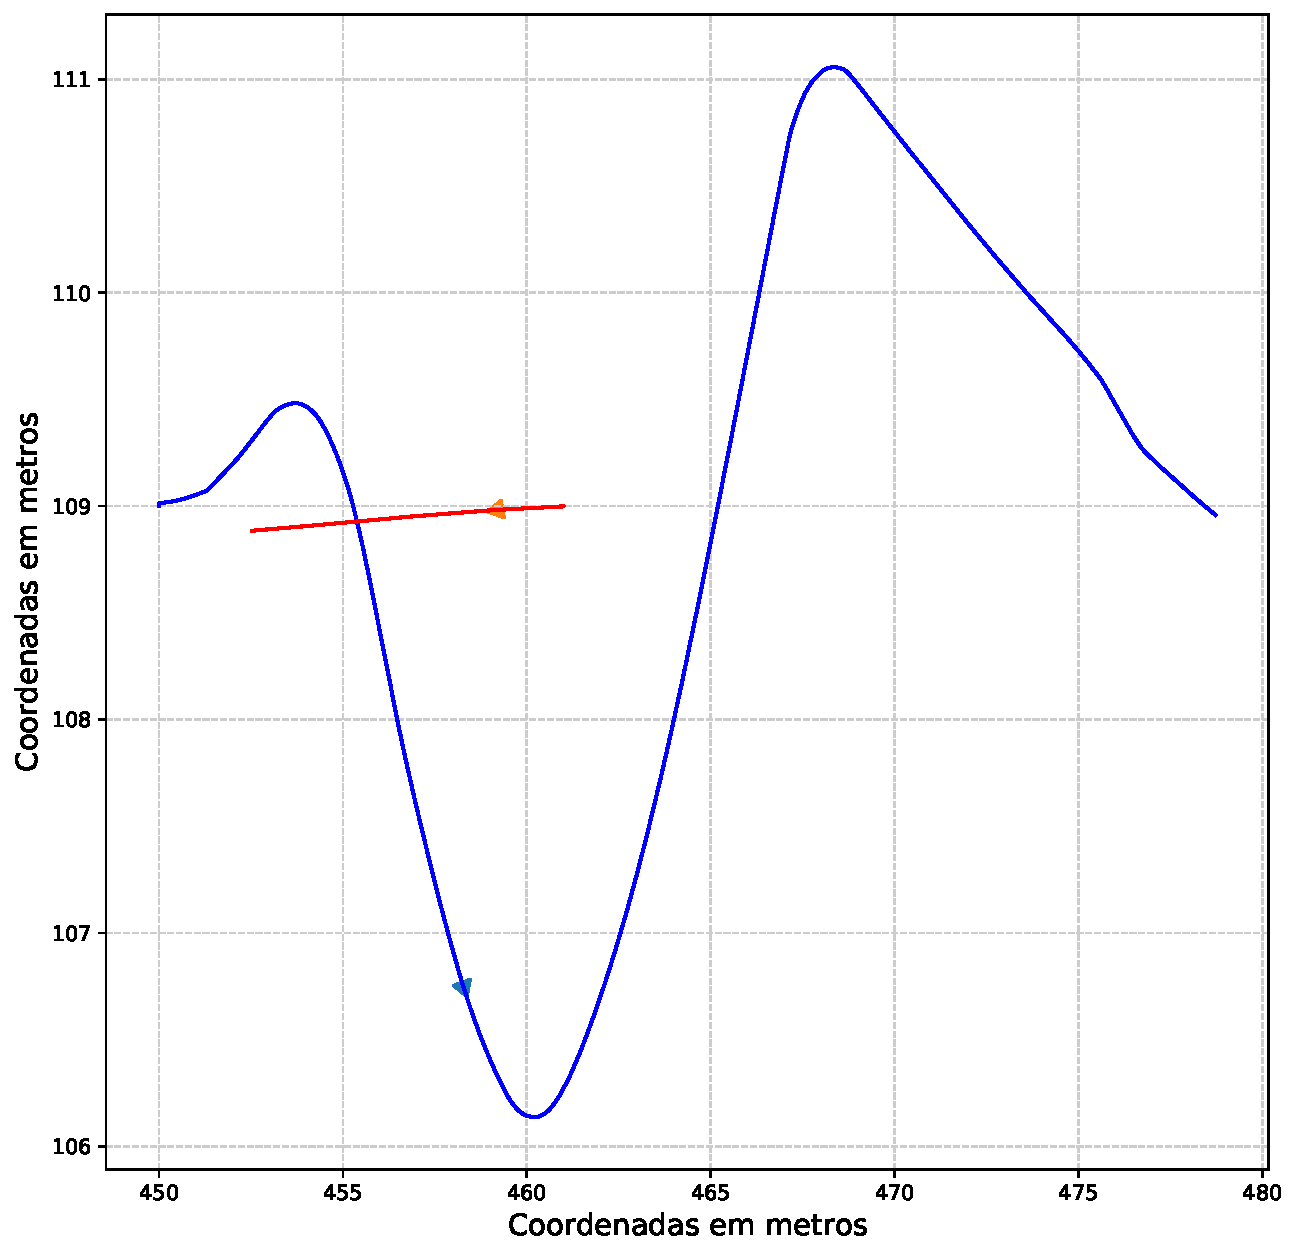
\includegraphics[scale=0.45]{fig/chap5/headon_cpa_trajectory.pdf}
            \caption{Trajeto das embarcações}
            \label{fig:chap5_headon_paths}
        \end{figure}
        
        \begin{figure}[H]
		\centering
% 		\begin{subfigure}{0.5\textwidth}
		\begin{subfigure}{1\textwidth}
            \centering
            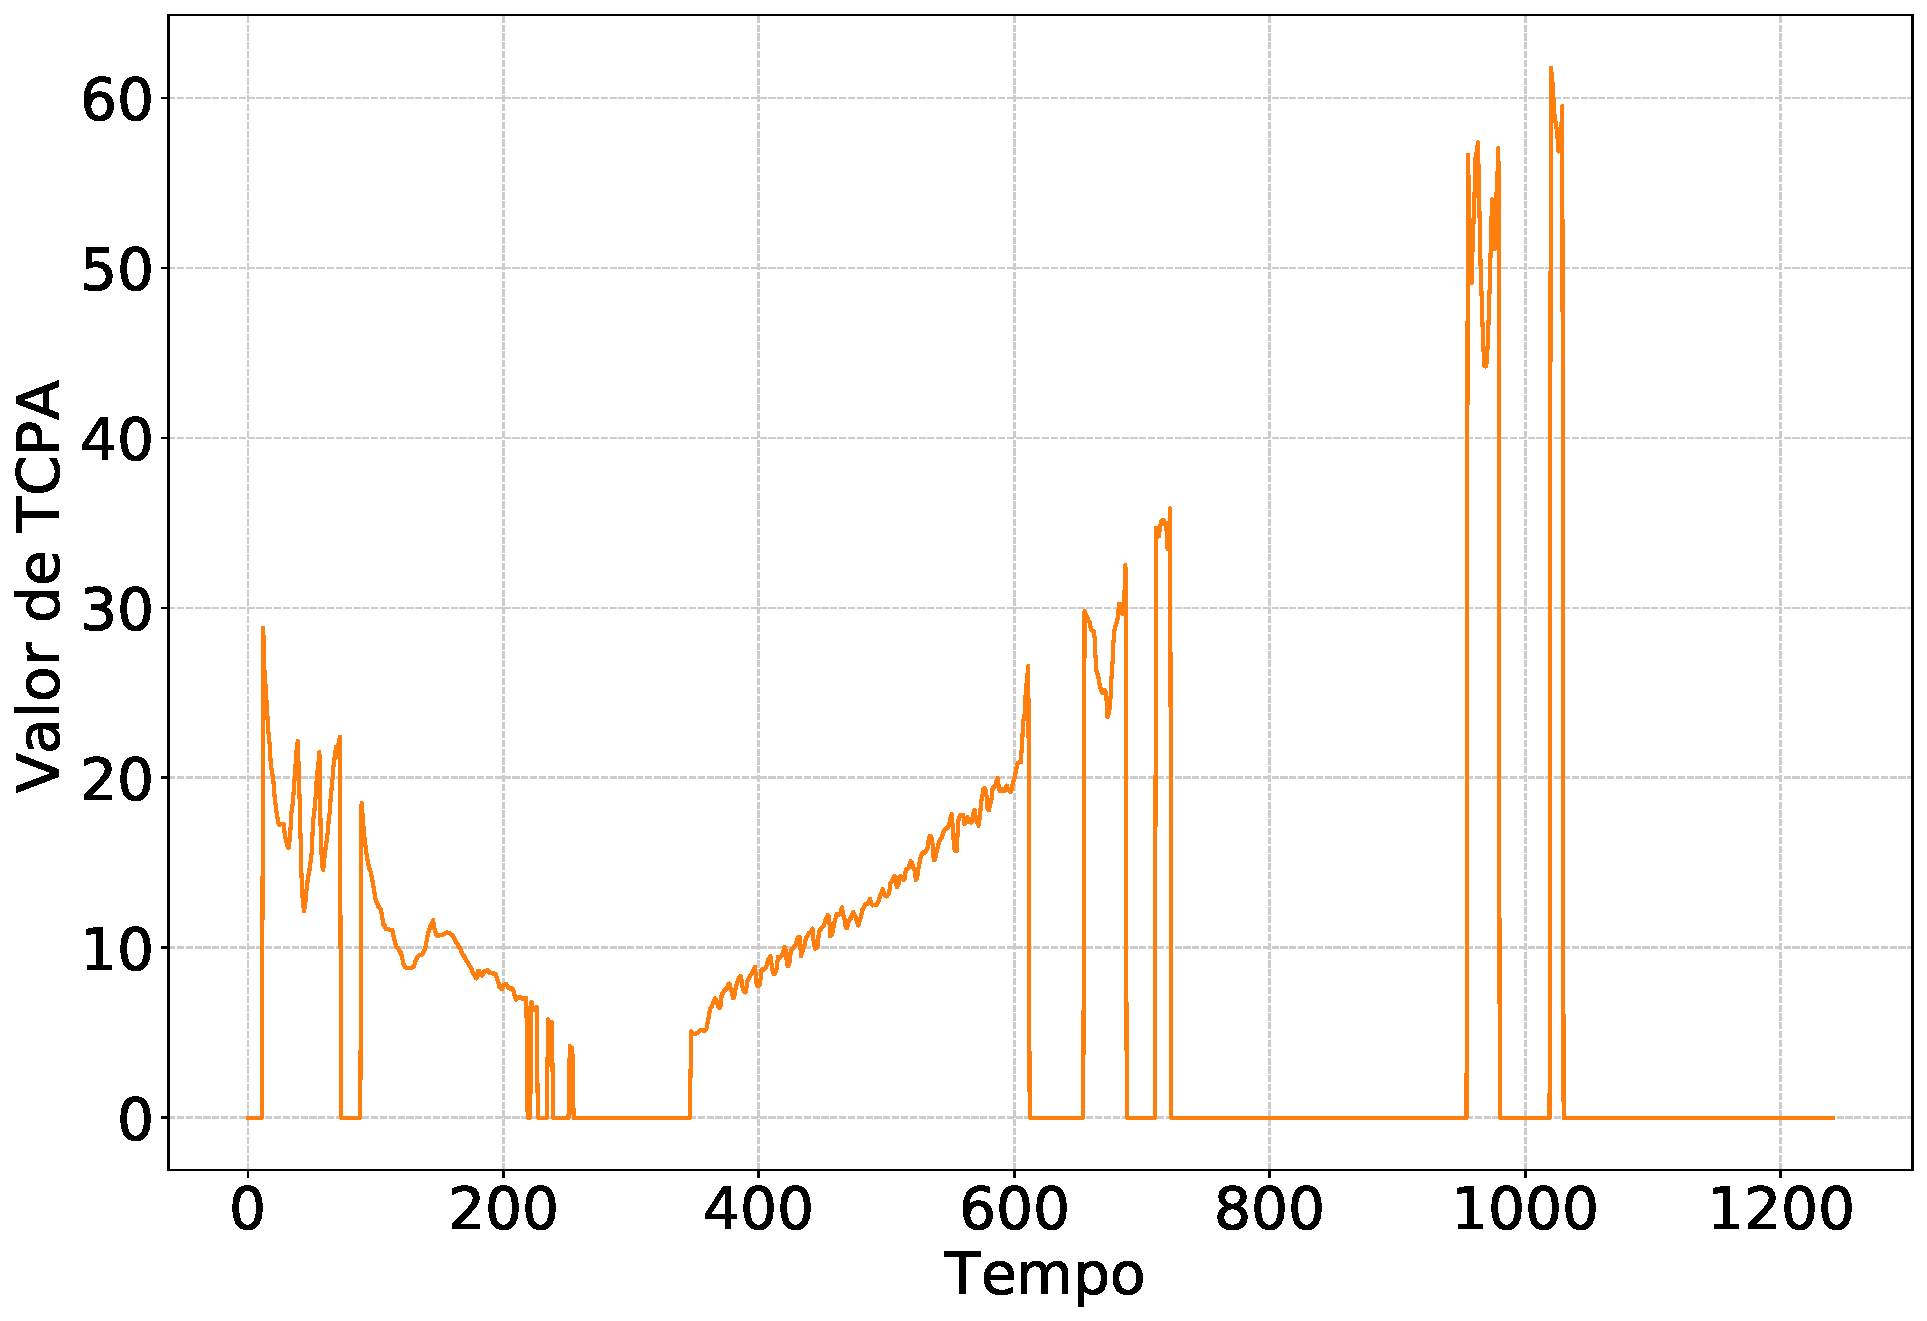
\includegraphics[width=\textwidth]{fig/chap5/headon_tcpa.pdf}
            \caption{TCPA}
            \label{fig:chap5_headon_tcpa}
        \end{subfigure}
% 		\begin{subfigure}{0.5\textwidth}
        \begin{subfigure}{1\textwidth}
            \centering
            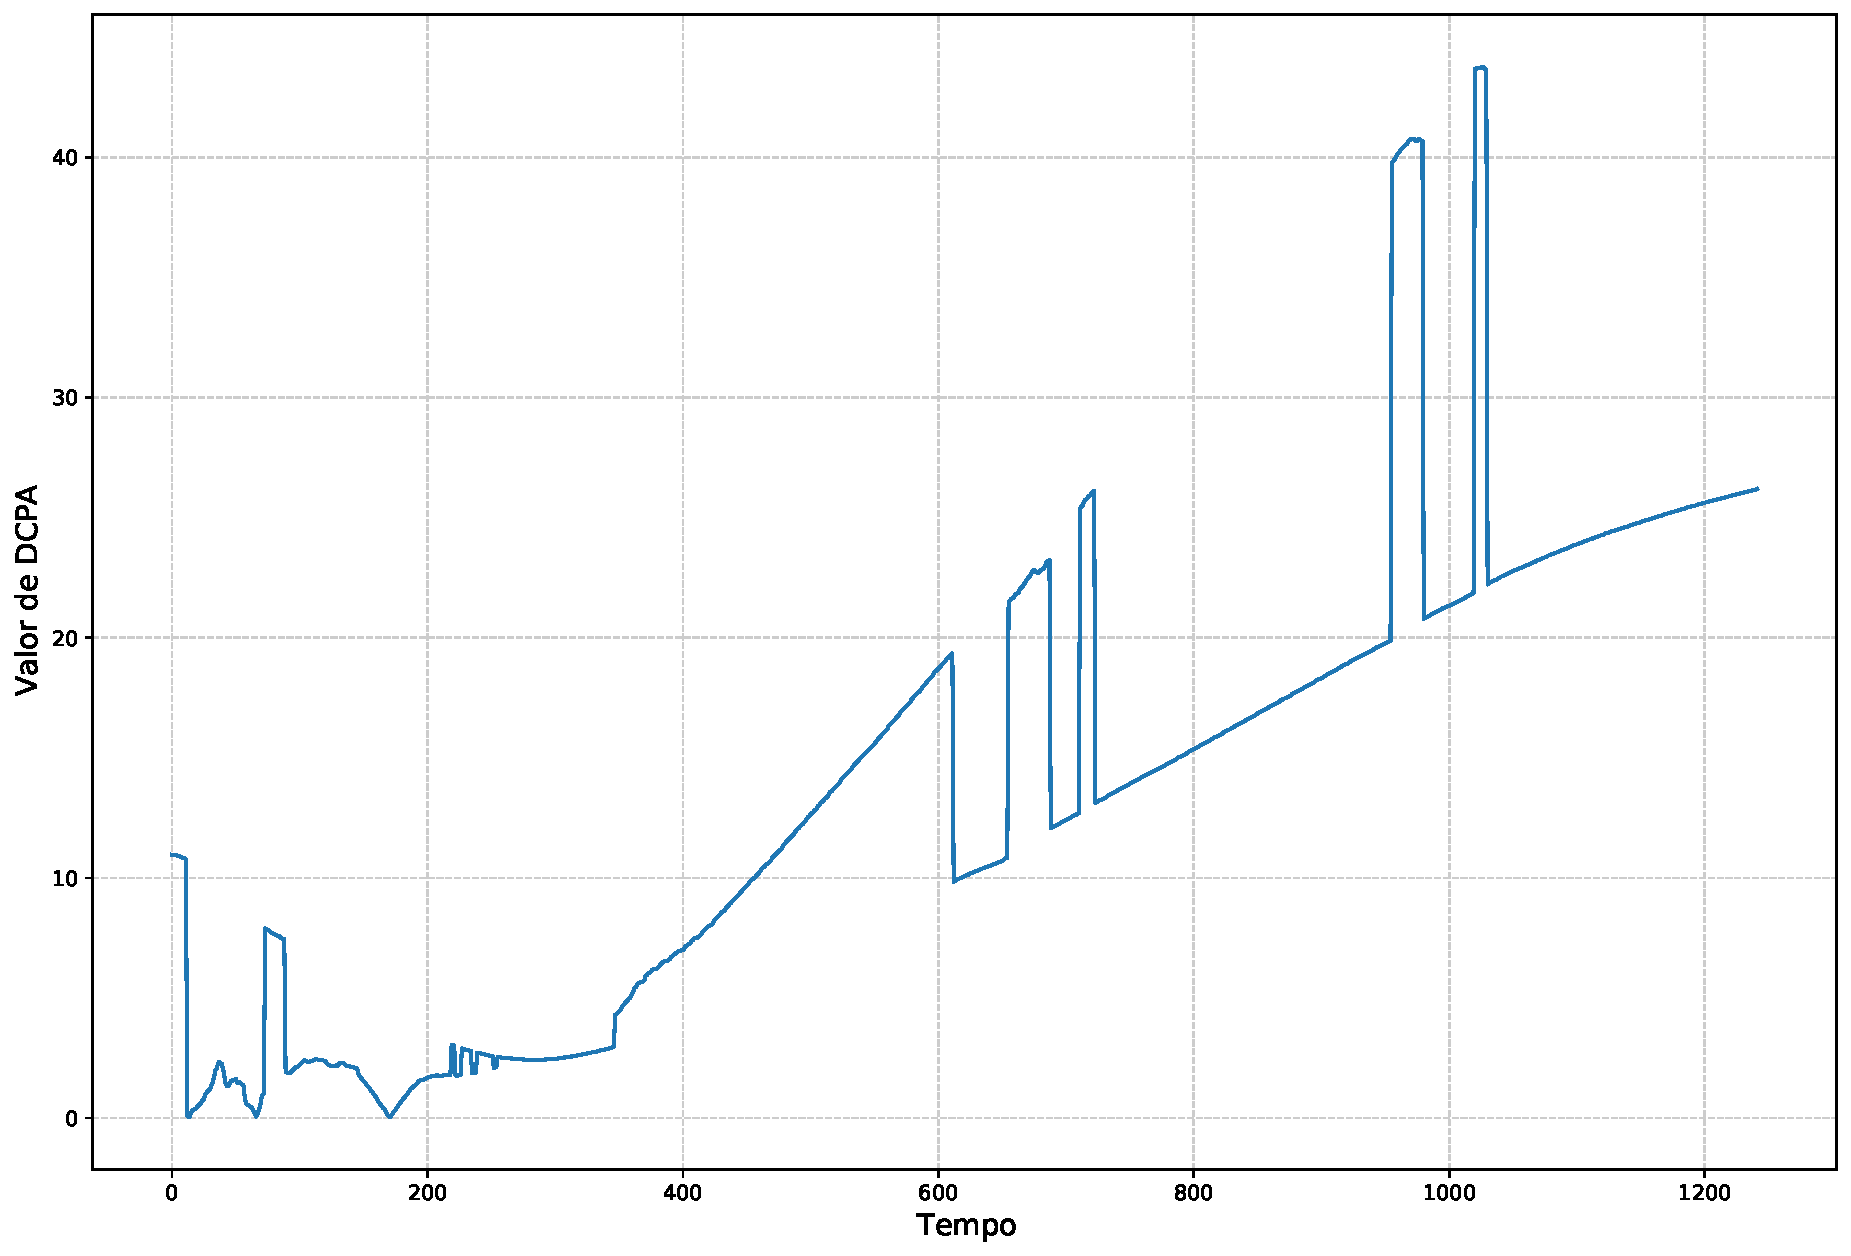
\includegraphics[width=\textwidth]{fig/chap5/headon_dcpa.pdf}
            \caption{DCPA}
            \label{fig:chap5_headon_dcpa}
        \end{subfigure}
        
        \caption{Informações do CPA}
        \label{fig:chap5_headon_cpa}
        \end{figure}
        
        \begin{figure}[H]
            \centering
            % 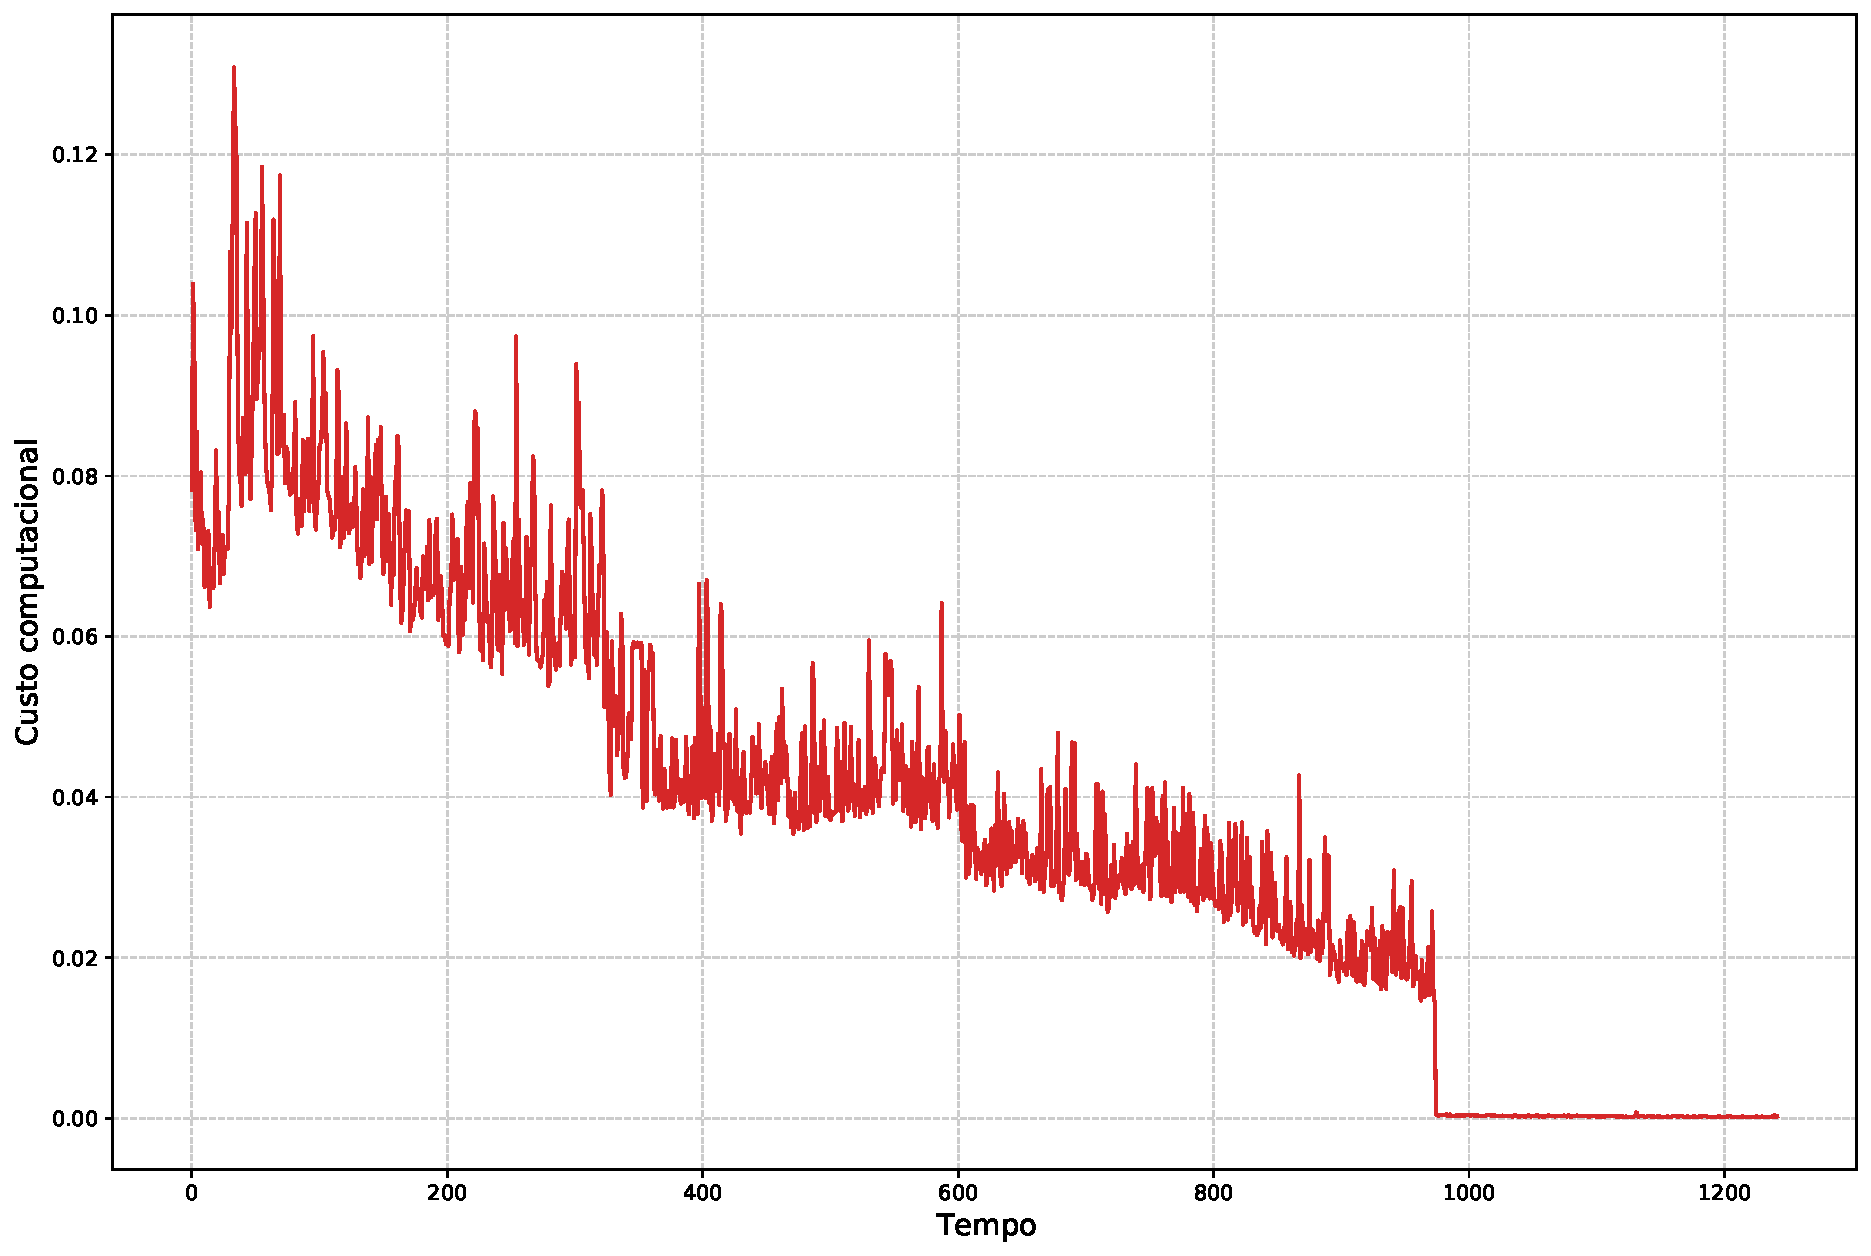
\includegraphics[width=0.3\textwidth]{fig/chap5/headon_computation_time.pdf}
            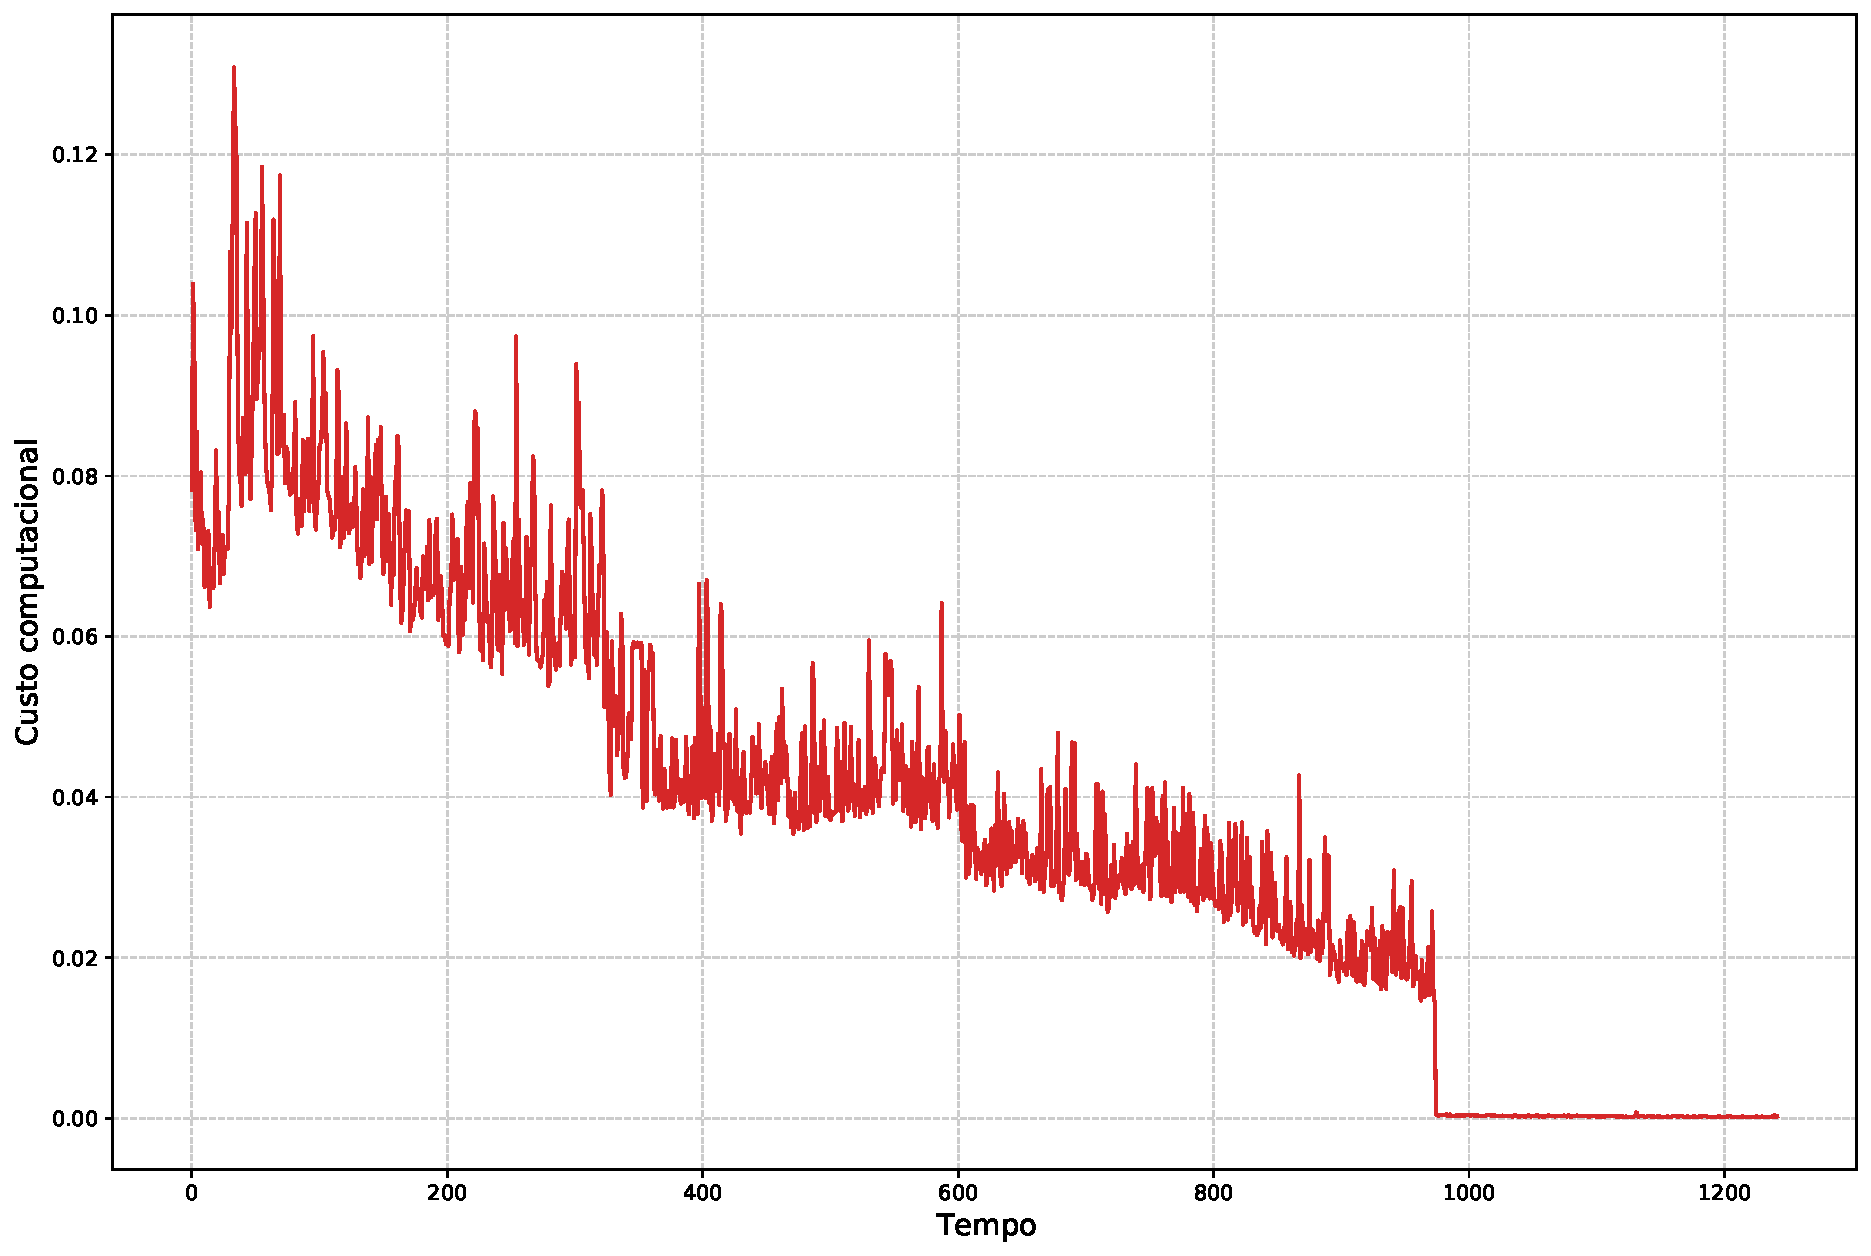
\includegraphics[width=\textwidth]{fig/chap5/headon_computation_time.pdf}
            \caption{Tempo de computação}
            \label{fig:chap5_headon_computation_time}
        \end{figure}
        
    \section{Overtake} \label{subchap5_overtake}
        A Figura~\ref{fig:chap5_overtake_paths} mostra o trajeto resultante para o caso de teste \textit{"Overtake"}. Nesse caso, as embarcações se deslocam na mesma direção e o USV realiza a manobra para ultrapassar a outra embarcação. A linha azul representa o trajeto realizado pelo USV enquanto que a linha vermelha representa o trajeto realizado pela outra embarcação. Os pequenos triângulos, em cada uma das trajetórias no gráfico, indicam o sentido em que as embarcações se deslocaram e a posição em que cada embarcação estava no momento em que foi registrada a menor distância entre elas durante todo o teste. Nesse caso, a distância foi de 2,255m. A Figura~\ref{fig:chap5_overtake_cpa} mostra as informações do CPA coletadas durante o teste. A análise da Figura~\ref{fig:chap5_overtake_tcpa} e da Figura~\ref{fig:chap5_overtake_dcpa} são análogas às análises realizadas na Seção~\ref{subchap5_headon}. Entretanto, é possível observar no início do gráfico, mostrado na Figura~\ref{fig:chap5_overtake_dcpa}, que houve um pico da estimativa de 
        distância, ocasionado pela decisão do USV de primeiro fazer uma curva para esquerda para só então executar o \textit{"Overtake"} pela direita da outra embarcação. A primeira conversão à esquerda é realizada pelo USV dado que, no início do teste, há um obstáculo estático à sua direita. Sua decisão em realizar o \textit{"Overtake"} pela direita se justifica pela COLREGS, que afirma que essa manobra deve ser realizada de forma que não configure novamente uma situação de \textit{"Overtake"}. A análise da Figura~\ref{fig:chap5_overtake_computation_time} é análoga à análise realizada anteriormente no Capítulo~\ref{subchap5_overtake}.
       
    
        \begin{figure}[H]
            \centering
            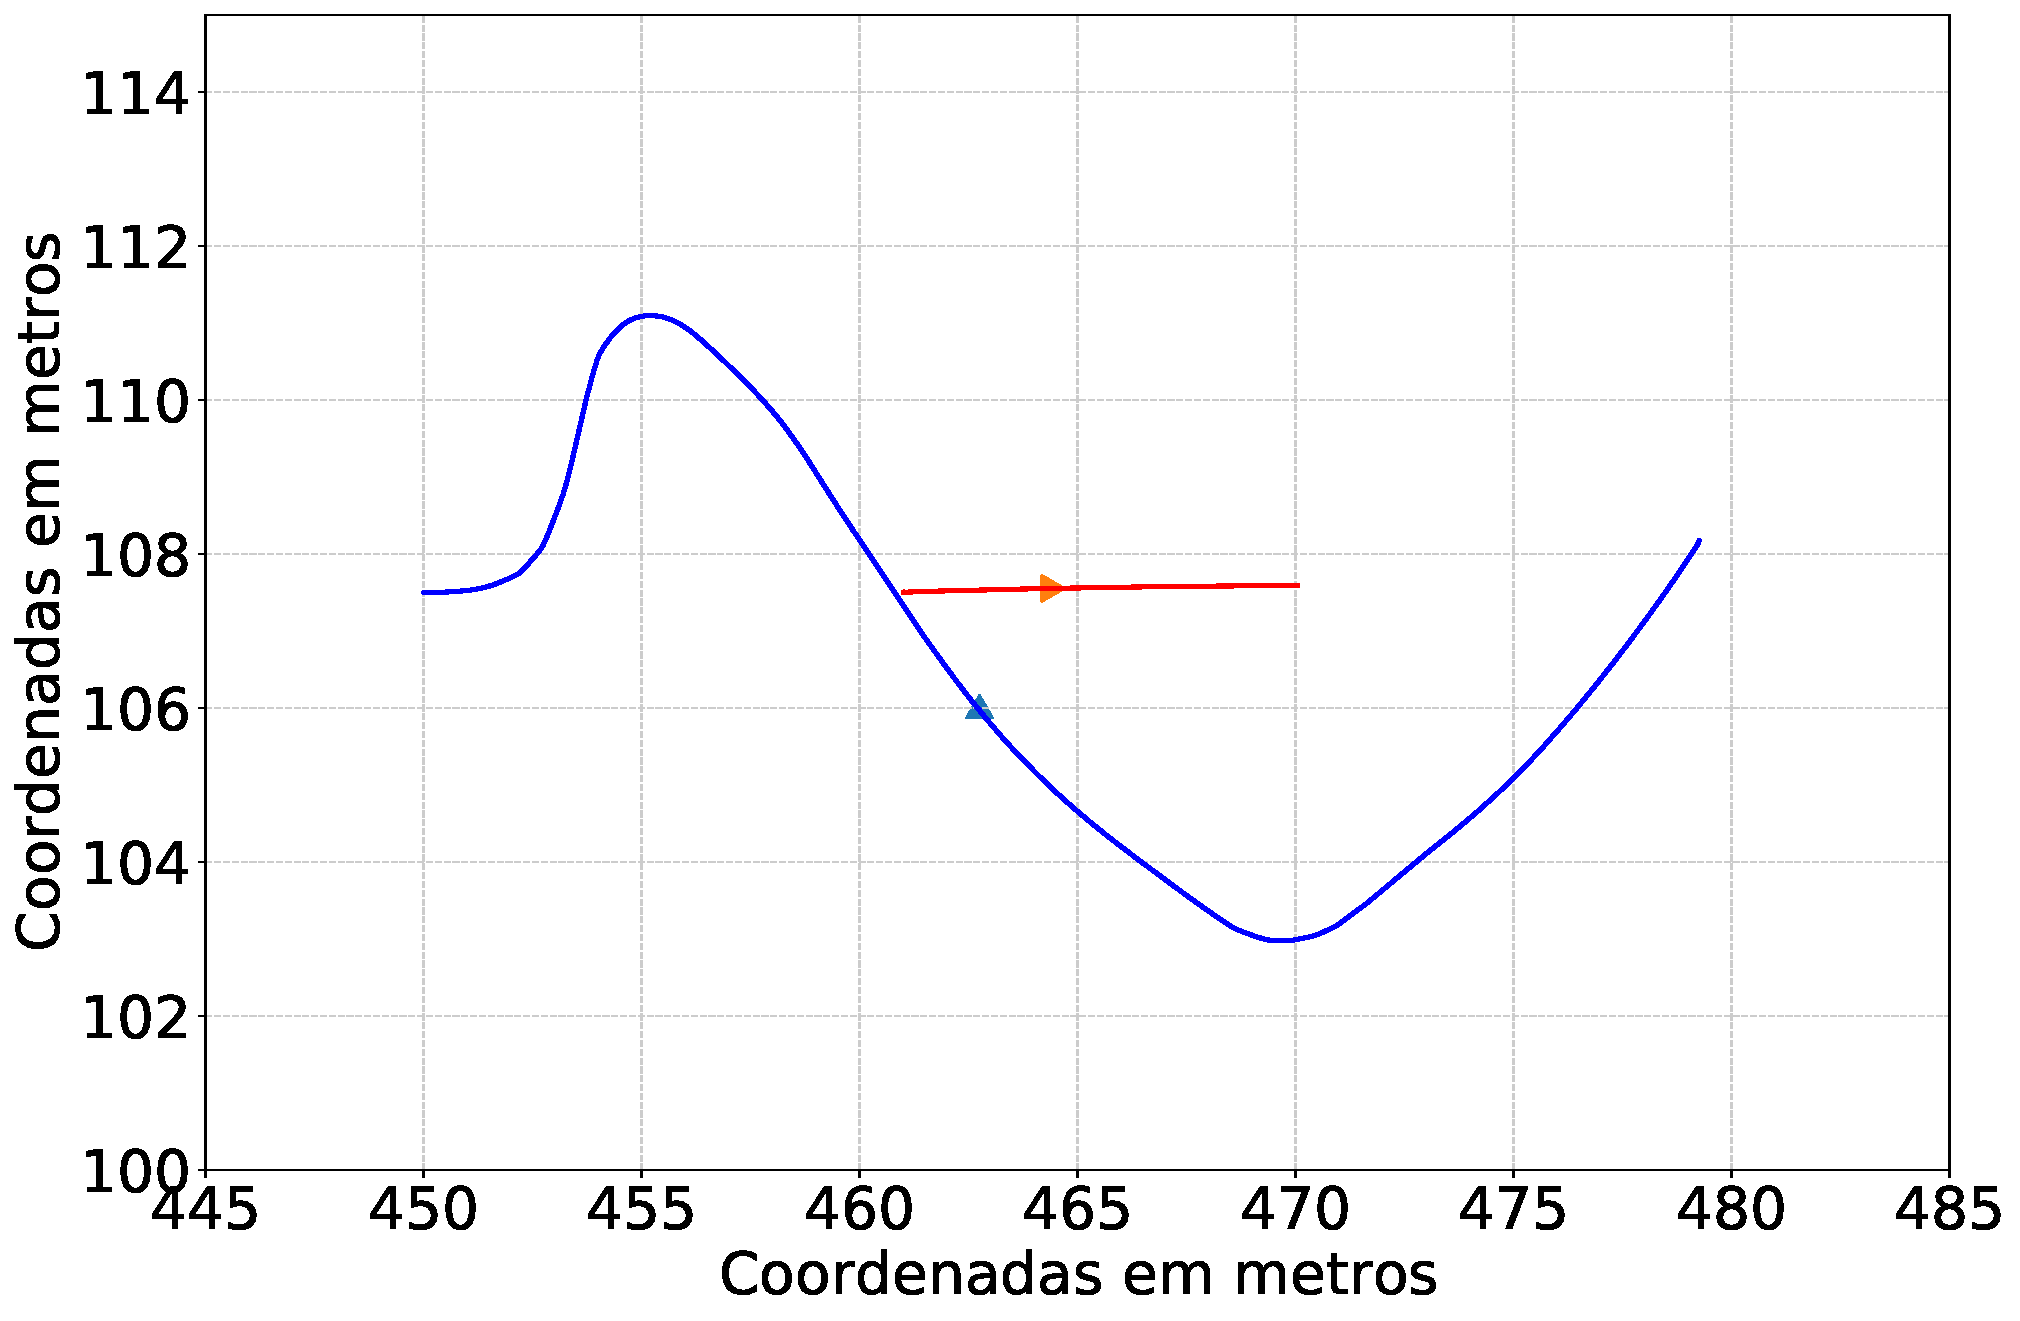
\includegraphics[scale=0.45]{fig/chap5/overtake_trajectory.pdf}
            \caption{Trajeto das embarcações}
            \label{fig:chap5_overtake_paths}
        \end{figure}
        
        \begin{figure}[H]
		\centering
% 		\begin{subfigure}{0.5\textwidth}
		\begin{subfigure}{1\textwidth}
            \centering
            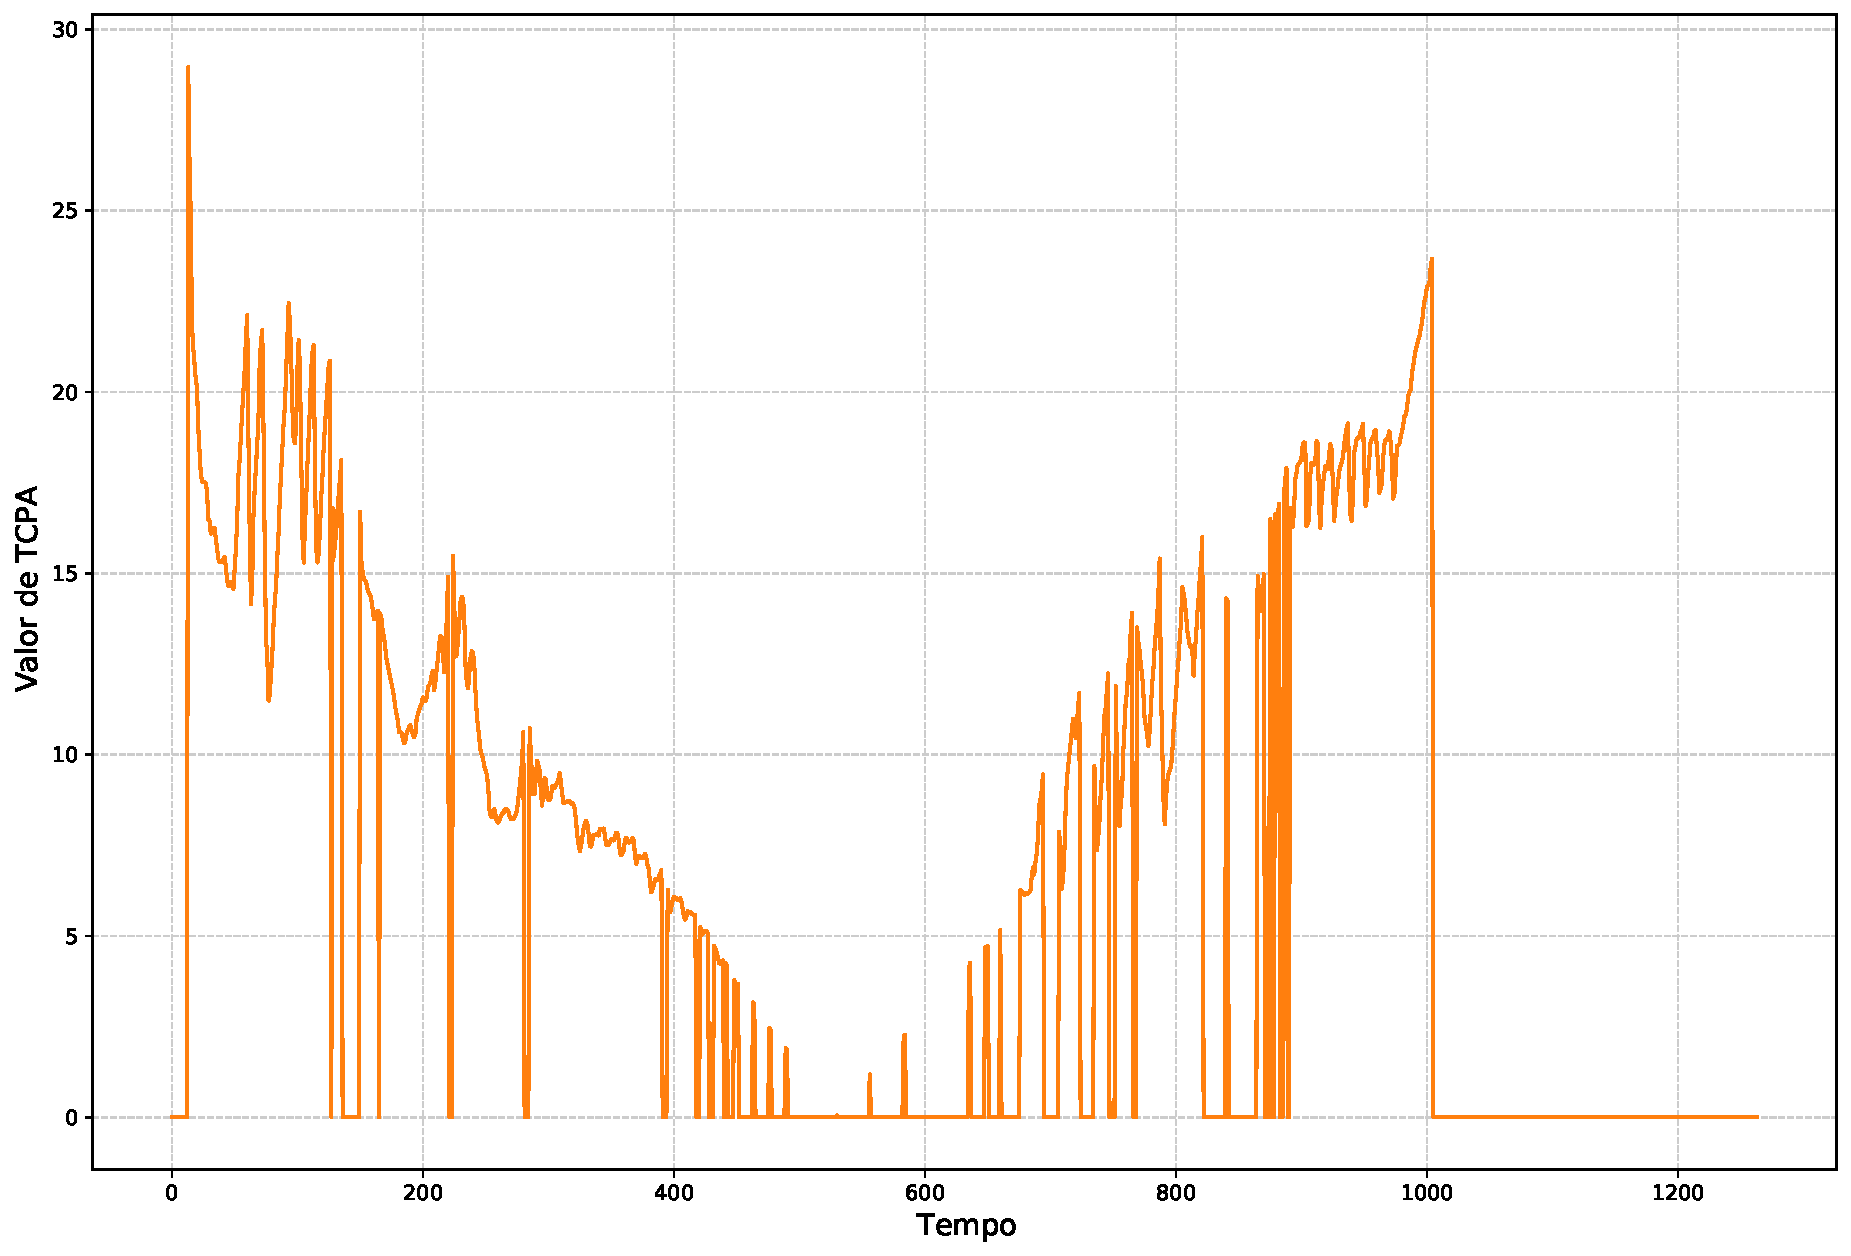
\includegraphics[width=\textwidth]{fig/chap5/overtake_tcpa.pdf}
            \caption{TCPA}
            \label{fig:chap5_overtake_tcpa}
        \end{subfigure}
% 		\begin{subfigure}{0.5\textwidth}
        \begin{subfigure}{1\textwidth}
            \centering
            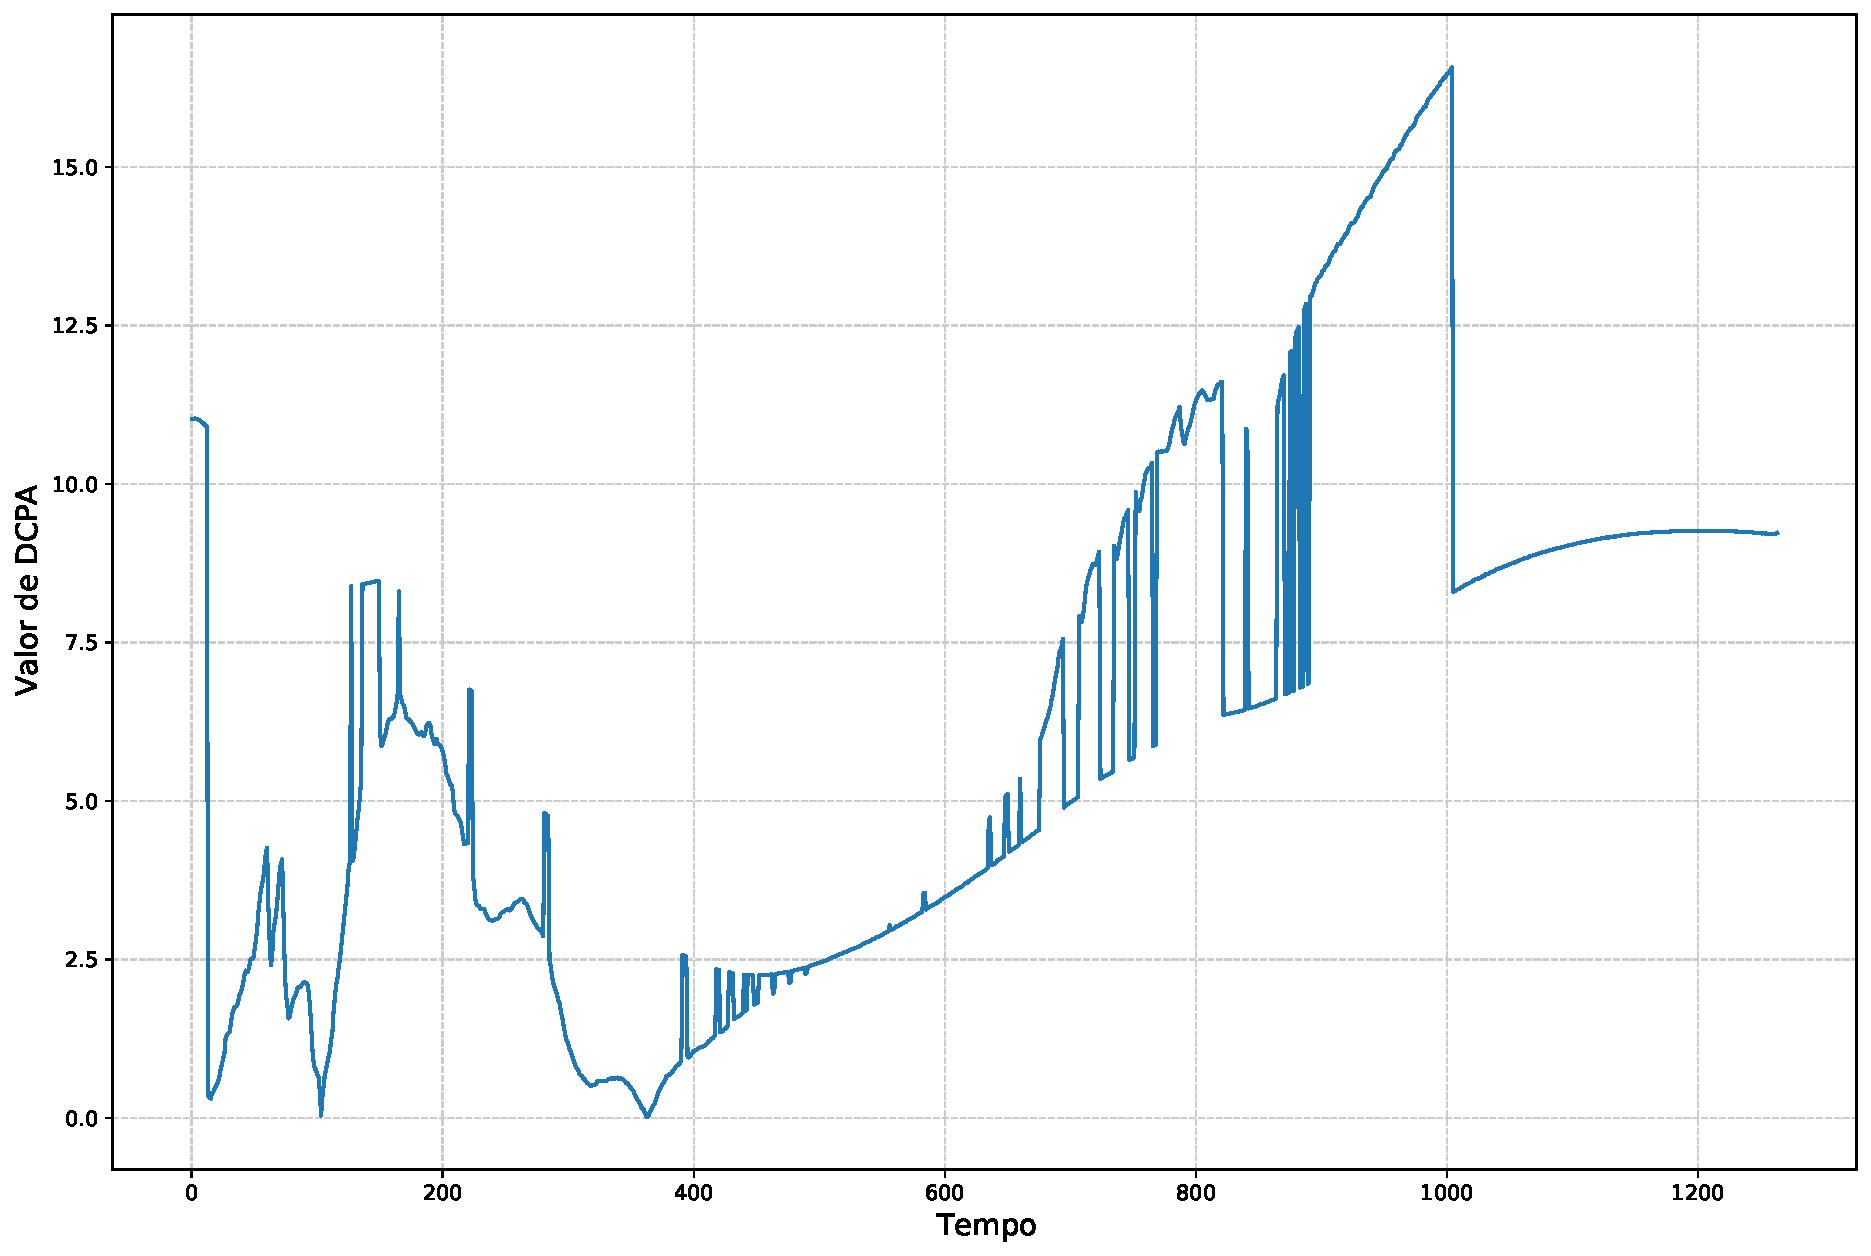
\includegraphics[width=\textwidth]{fig/chap5/overtake_dcpa.pdf}
            \caption{DCPA}
            \label{fig:chap5_overtake_dcpa}
        \end{subfigure}
        
        \caption{Informações do CPA}
        \label{fig:chap5_overtake_cpa}
        \end{figure}
        
        \begin{figure}[H]
            \centering
            % 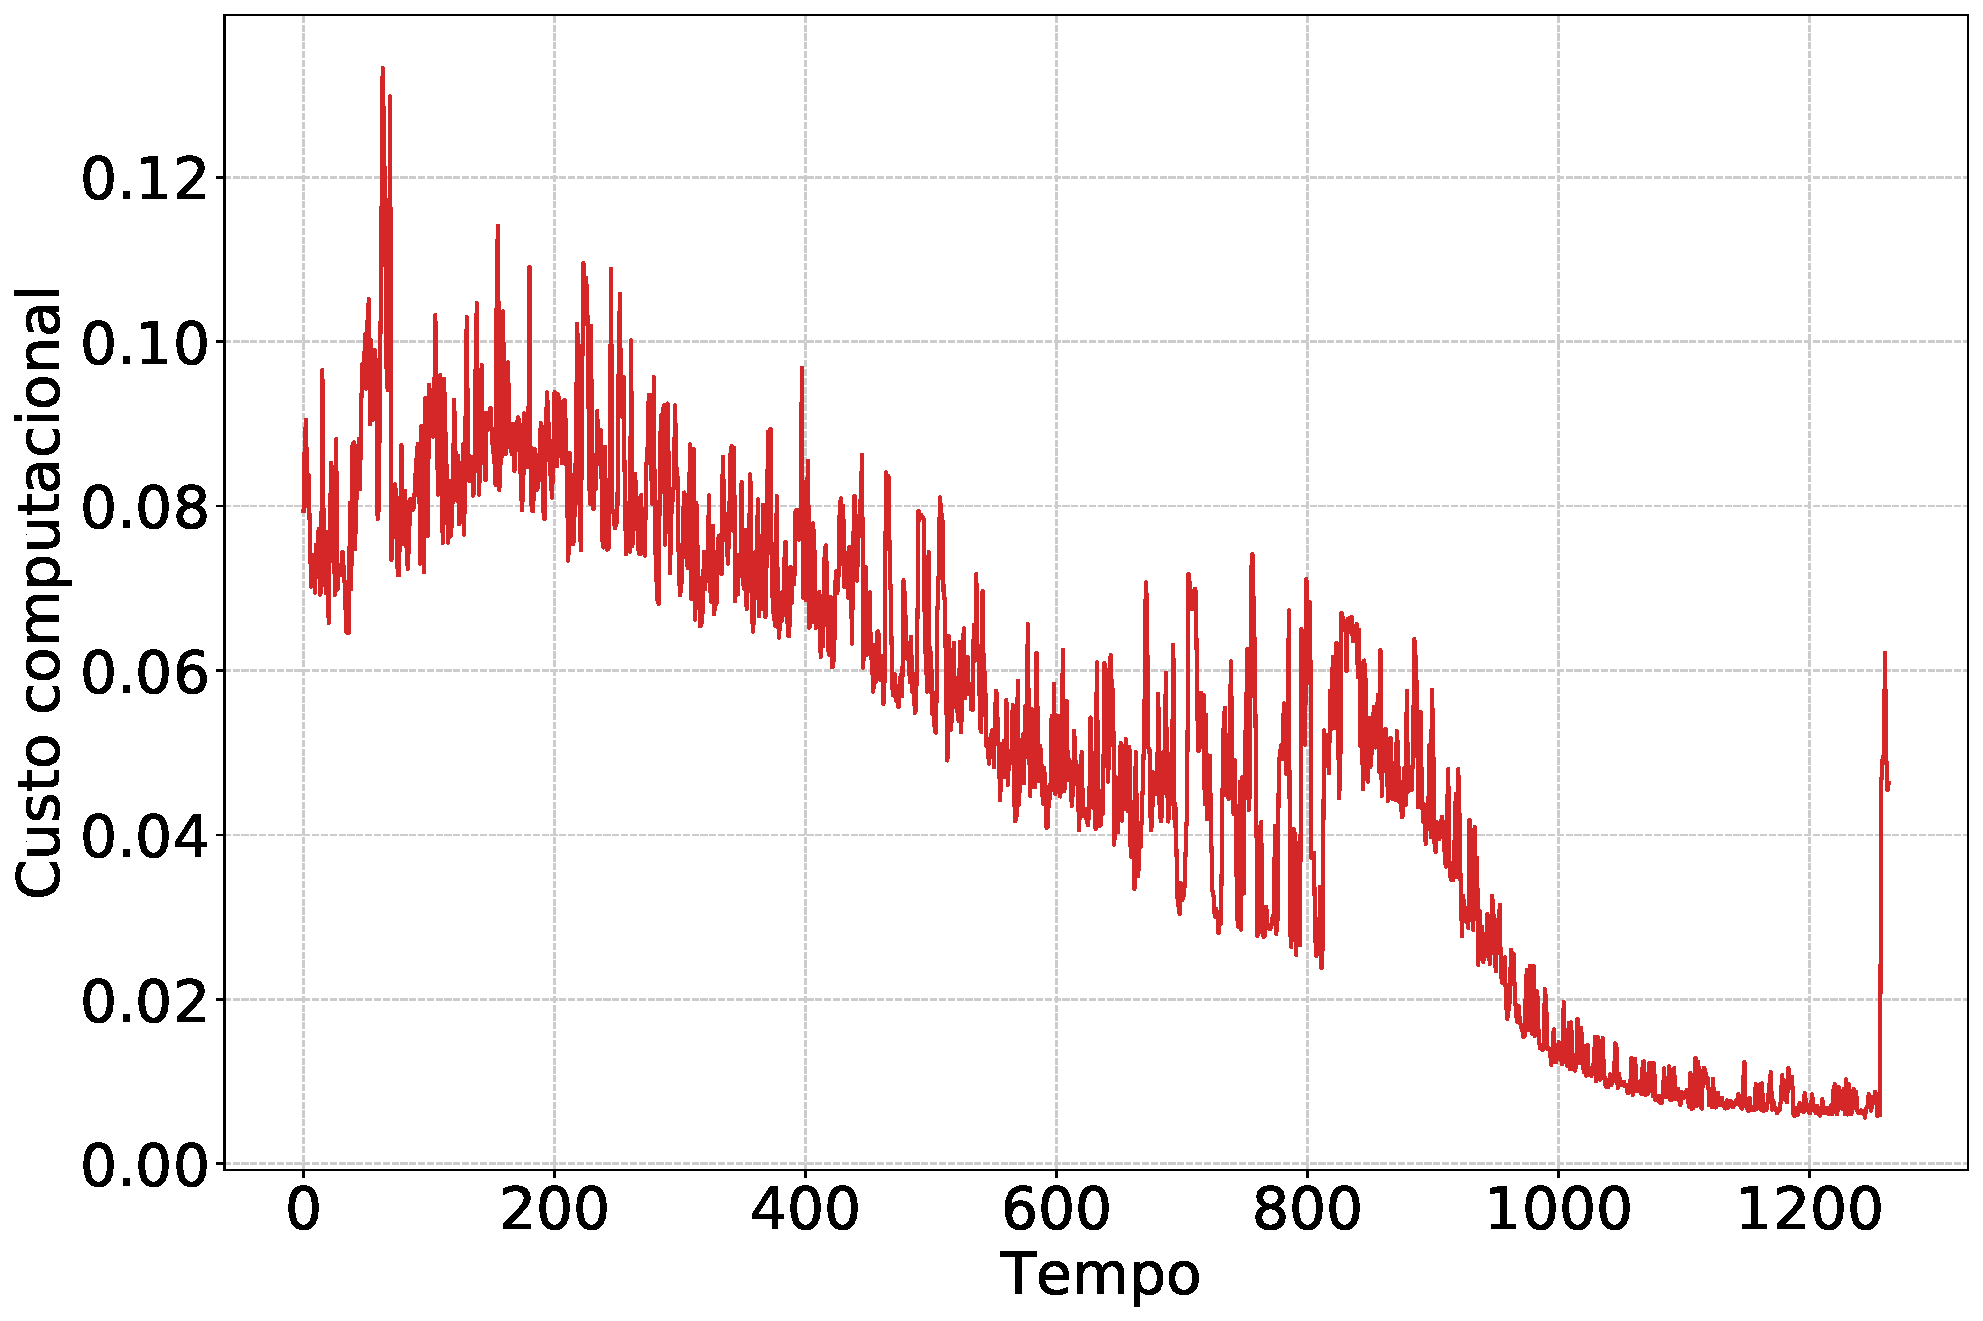
\includegraphics[width=0.3\textwidth]{fig/chap5/overtake_computation_time.pdf}
            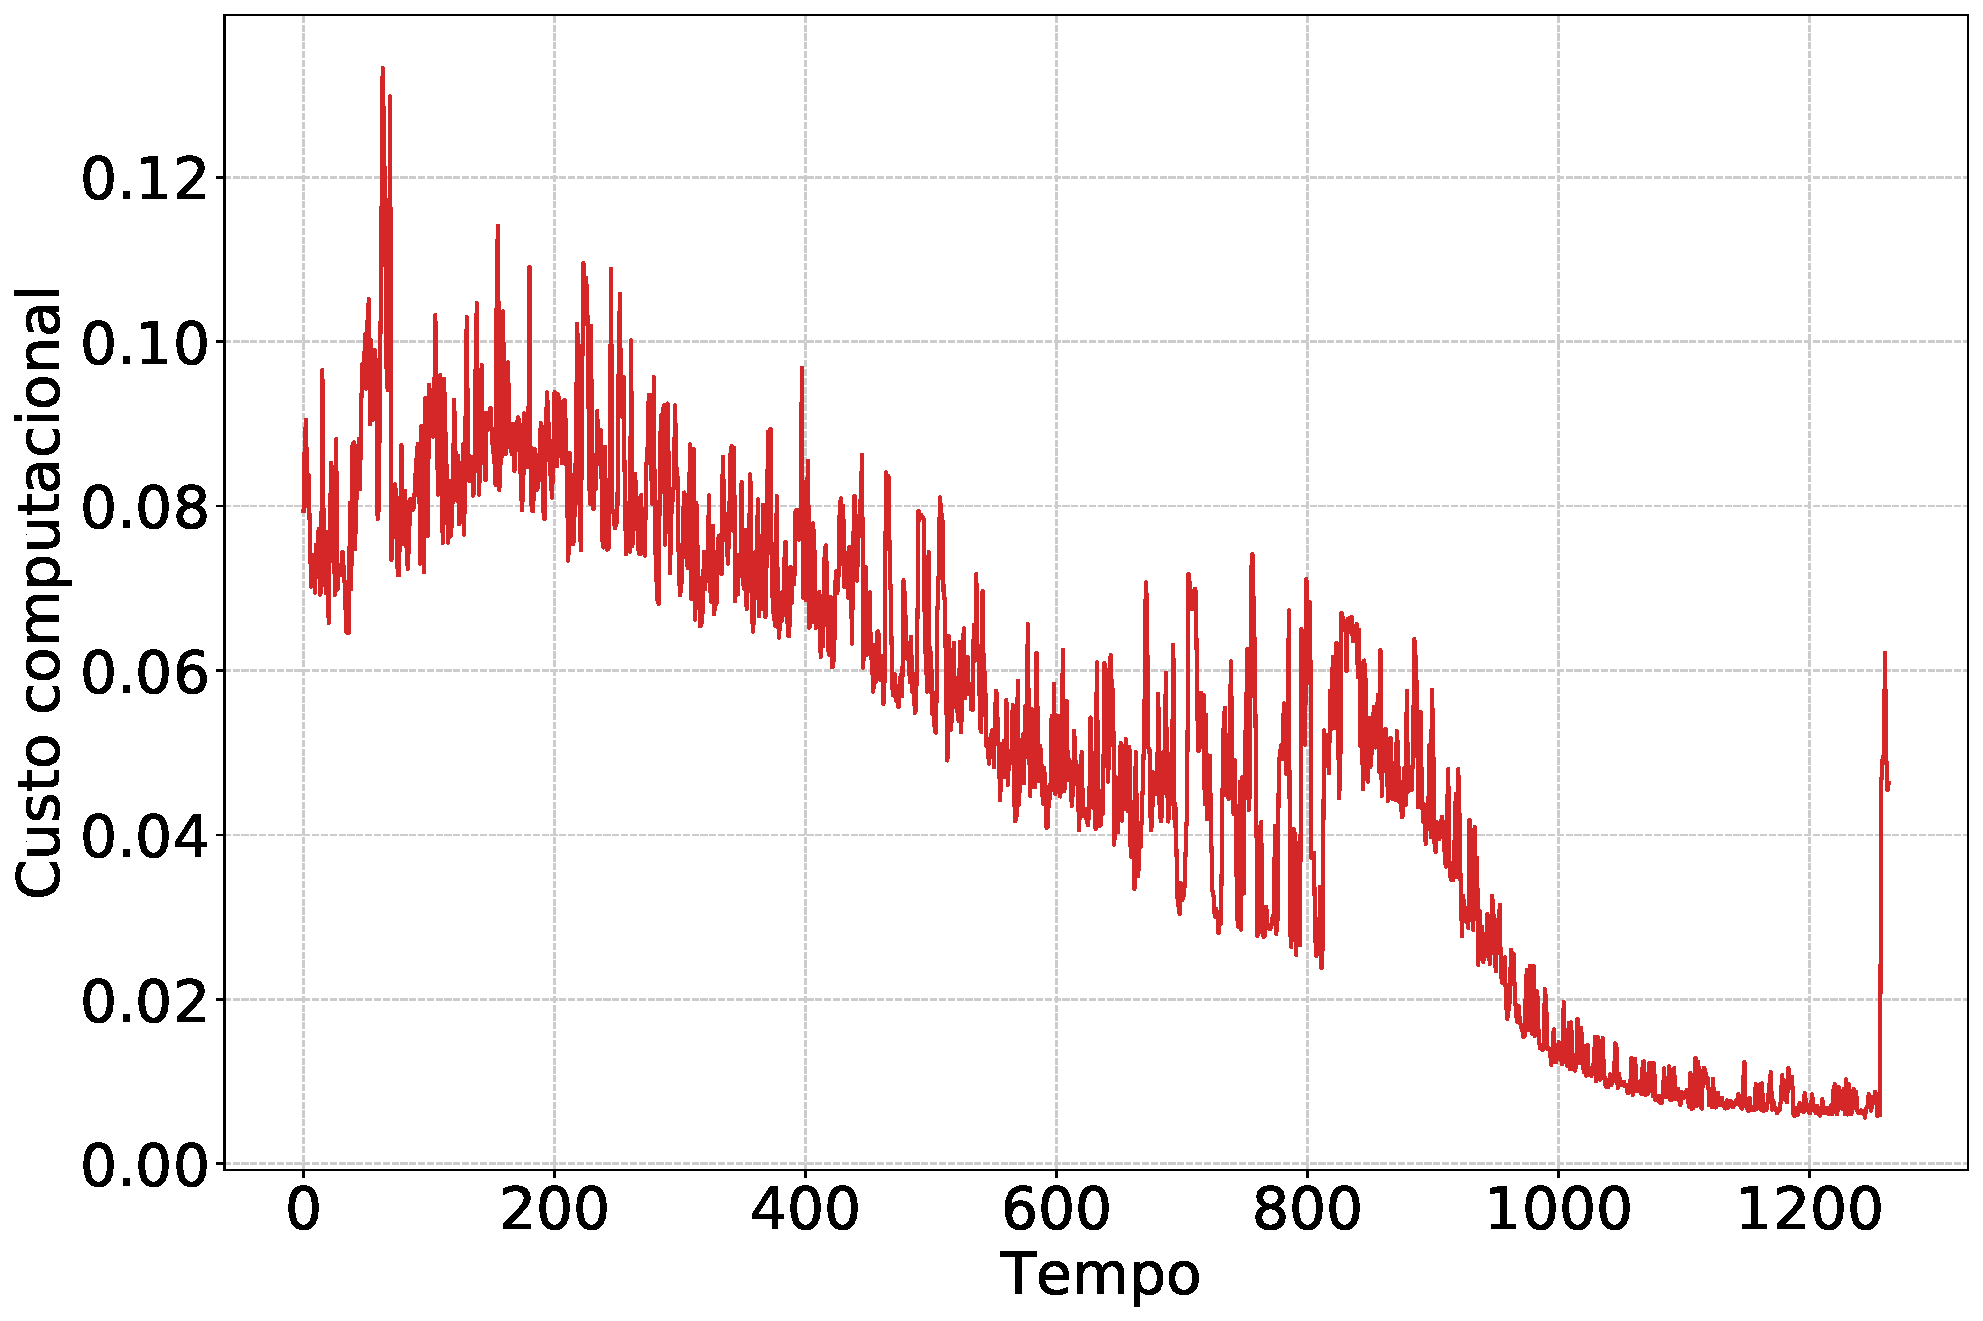
\includegraphics[width=\textwidth]{fig/chap5/overtake_computation_time.pdf}
            \caption{Tempo de computação}
            \label{fig:chap5_overtake_computation_time}
        \end{figure}
        
    \section{Crossing from Left} \label{subchap5_crossing_from_left}
        A Figura~\ref{fig:chap5_crossing_left_paths} mostra a trajetória resultante das embarcações para o caso de teste \textit{"Crossing from Left"}, onde o USV encontra a outra embarcação à sua esquerda. Nesse caso, segundo a COLREGS, o USV não é responsável por evitar a colisão em caso de risco. Novamente, a linha azul na Figura~\ref{fig:chap5_crossing_left_paths} indica o trajeto realizado pelo USV enquanto que a linha vermelha indica o trajeto realizado pela outra embarcação. Neste caso de teste a menor distância registrada entre as embarcações, indicado pelos triângulos vermelhos, foi de 8,316m. As análises do \tcpa e do \dcpa, ilustrados respectivamente na 
        Figura~\ref{fig:chap5_crossing_left_tcpa} e na Figura~\ref{fig:chap5_crossing_left_dcpa}, são análogas às análises realizadas anteriormente, em que com as embarcações se aproximando a tendência é que o \tcpa e o \dcpa diminuam, enquanto que ao se afastarem esses valores tendem a aumentar. No gráfico do tempo de computação (Figura~\ref{fig:chap5_crossing_left_computation_time}), percebe-se que o esforço computacional é muito pequeno até o momento em que a outra embarcação é detectada pelo planejador local. Segundo Jurak~\cite{Jurak2020COLREGS}, um erro de conversão de coordenadas globais para locais ocasiona um objetivo inválido para o planejador local, ocasionando o vale apresentado na Figura~\ref{fig:chap5_crossing_left_computation_time}. Pois segundo o fluxograma apresentado no 
        Capítulo~\ref{chap4:desenvolvimento}, se o objetivo do planejador local for inválido por dois ciclos de processamento, o sistema não deve fazer nada.
    
        \begin{figure}[H]
            \centering
            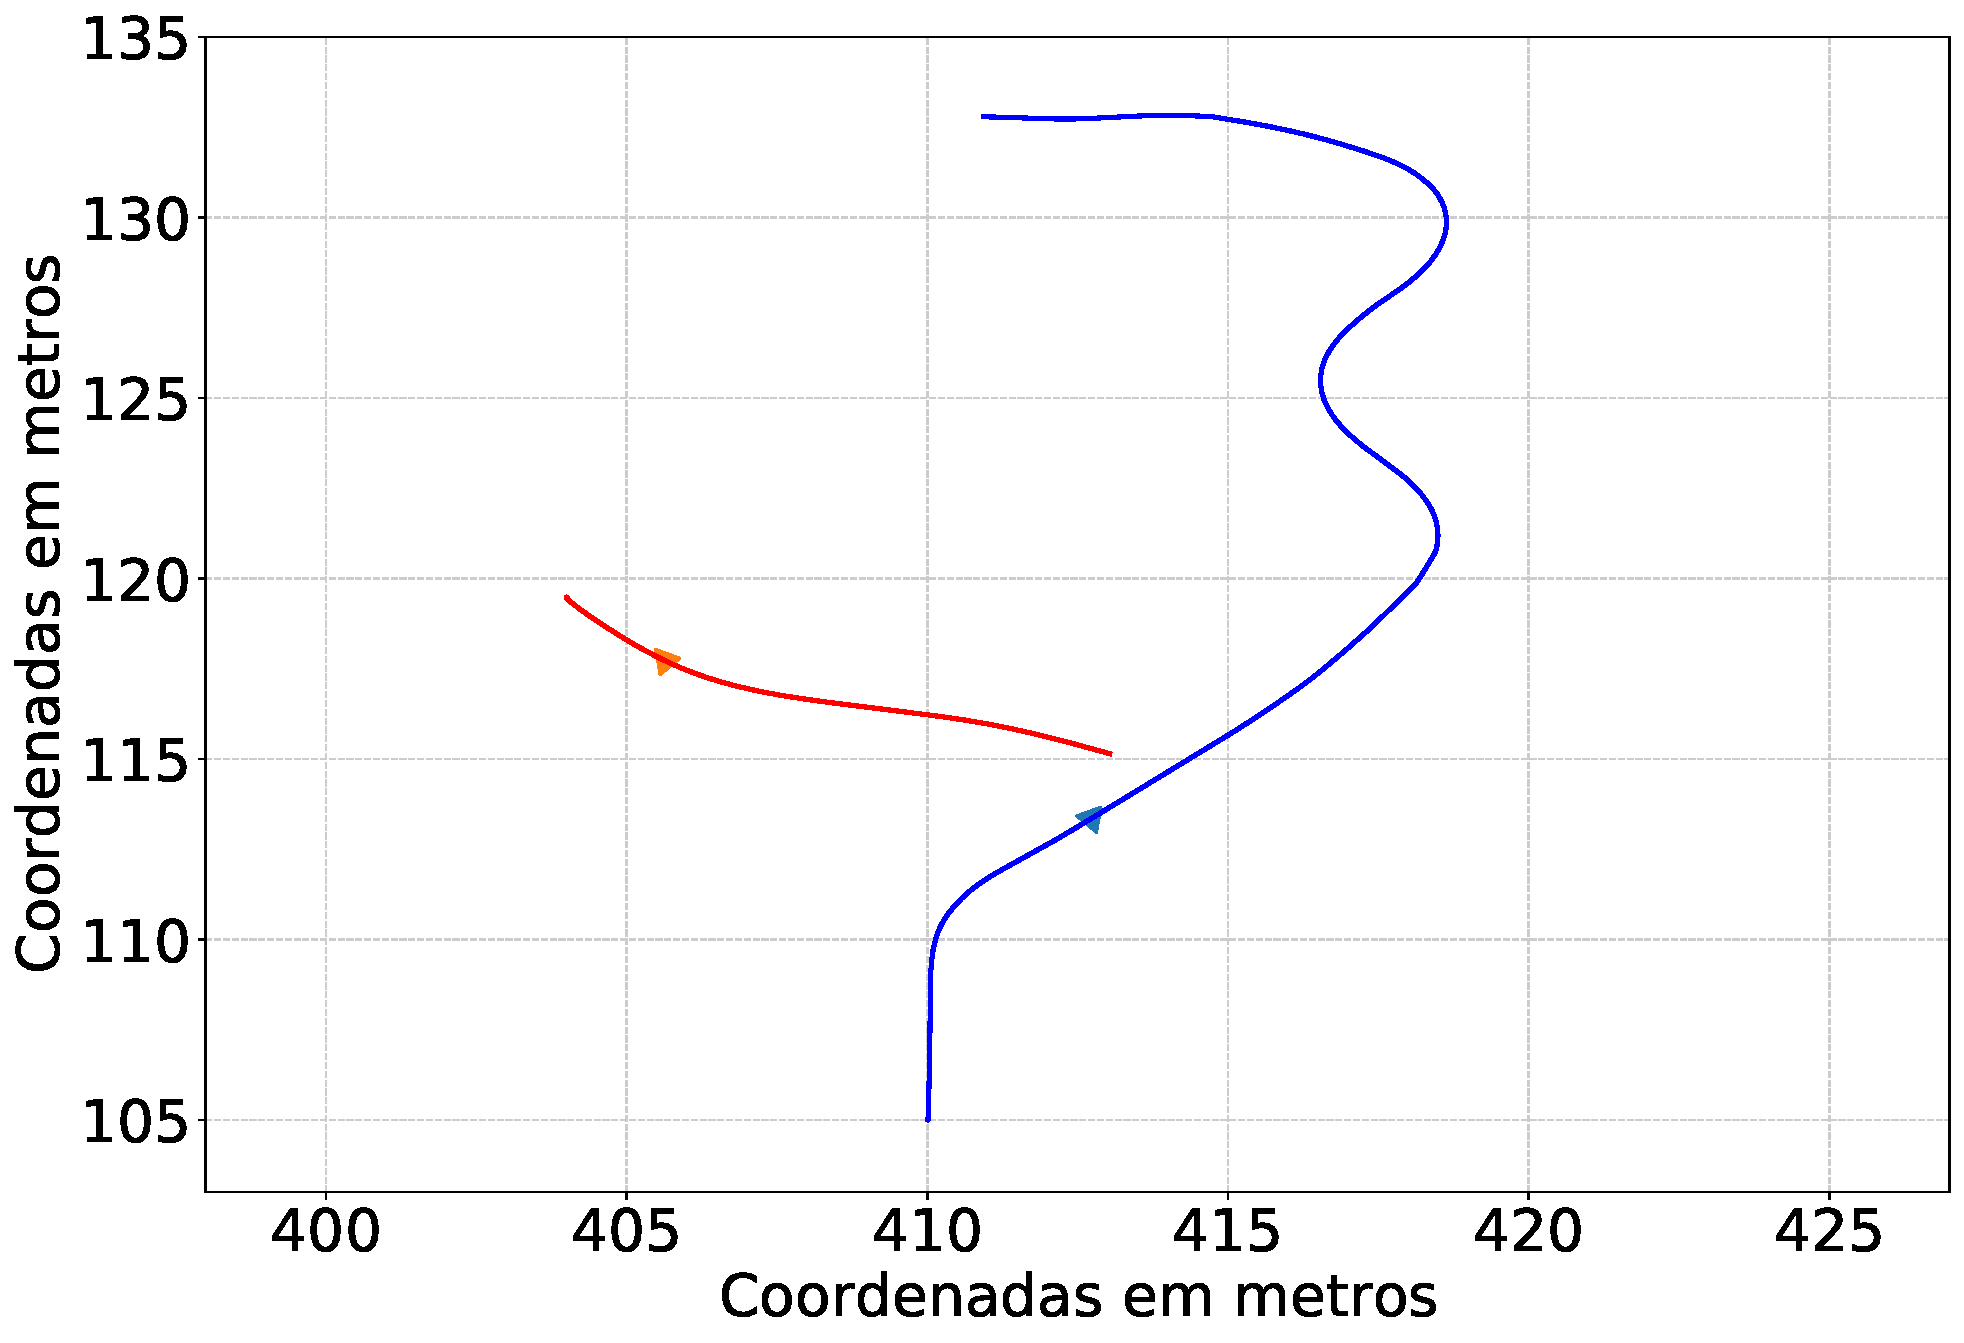
\includegraphics[scale=0.45]{fig/chap5/crossing_left_trajectory.pdf}
            \caption{Trajeto das embarcações}
            \label{fig:chap5_crossing_left_paths}
        \end{figure}
        
        \begin{figure}[H]
		\centering
% 		\begin{subfigure}{0.5\textwidth}
		\begin{subfigure}{1\textwidth}
            \centering
            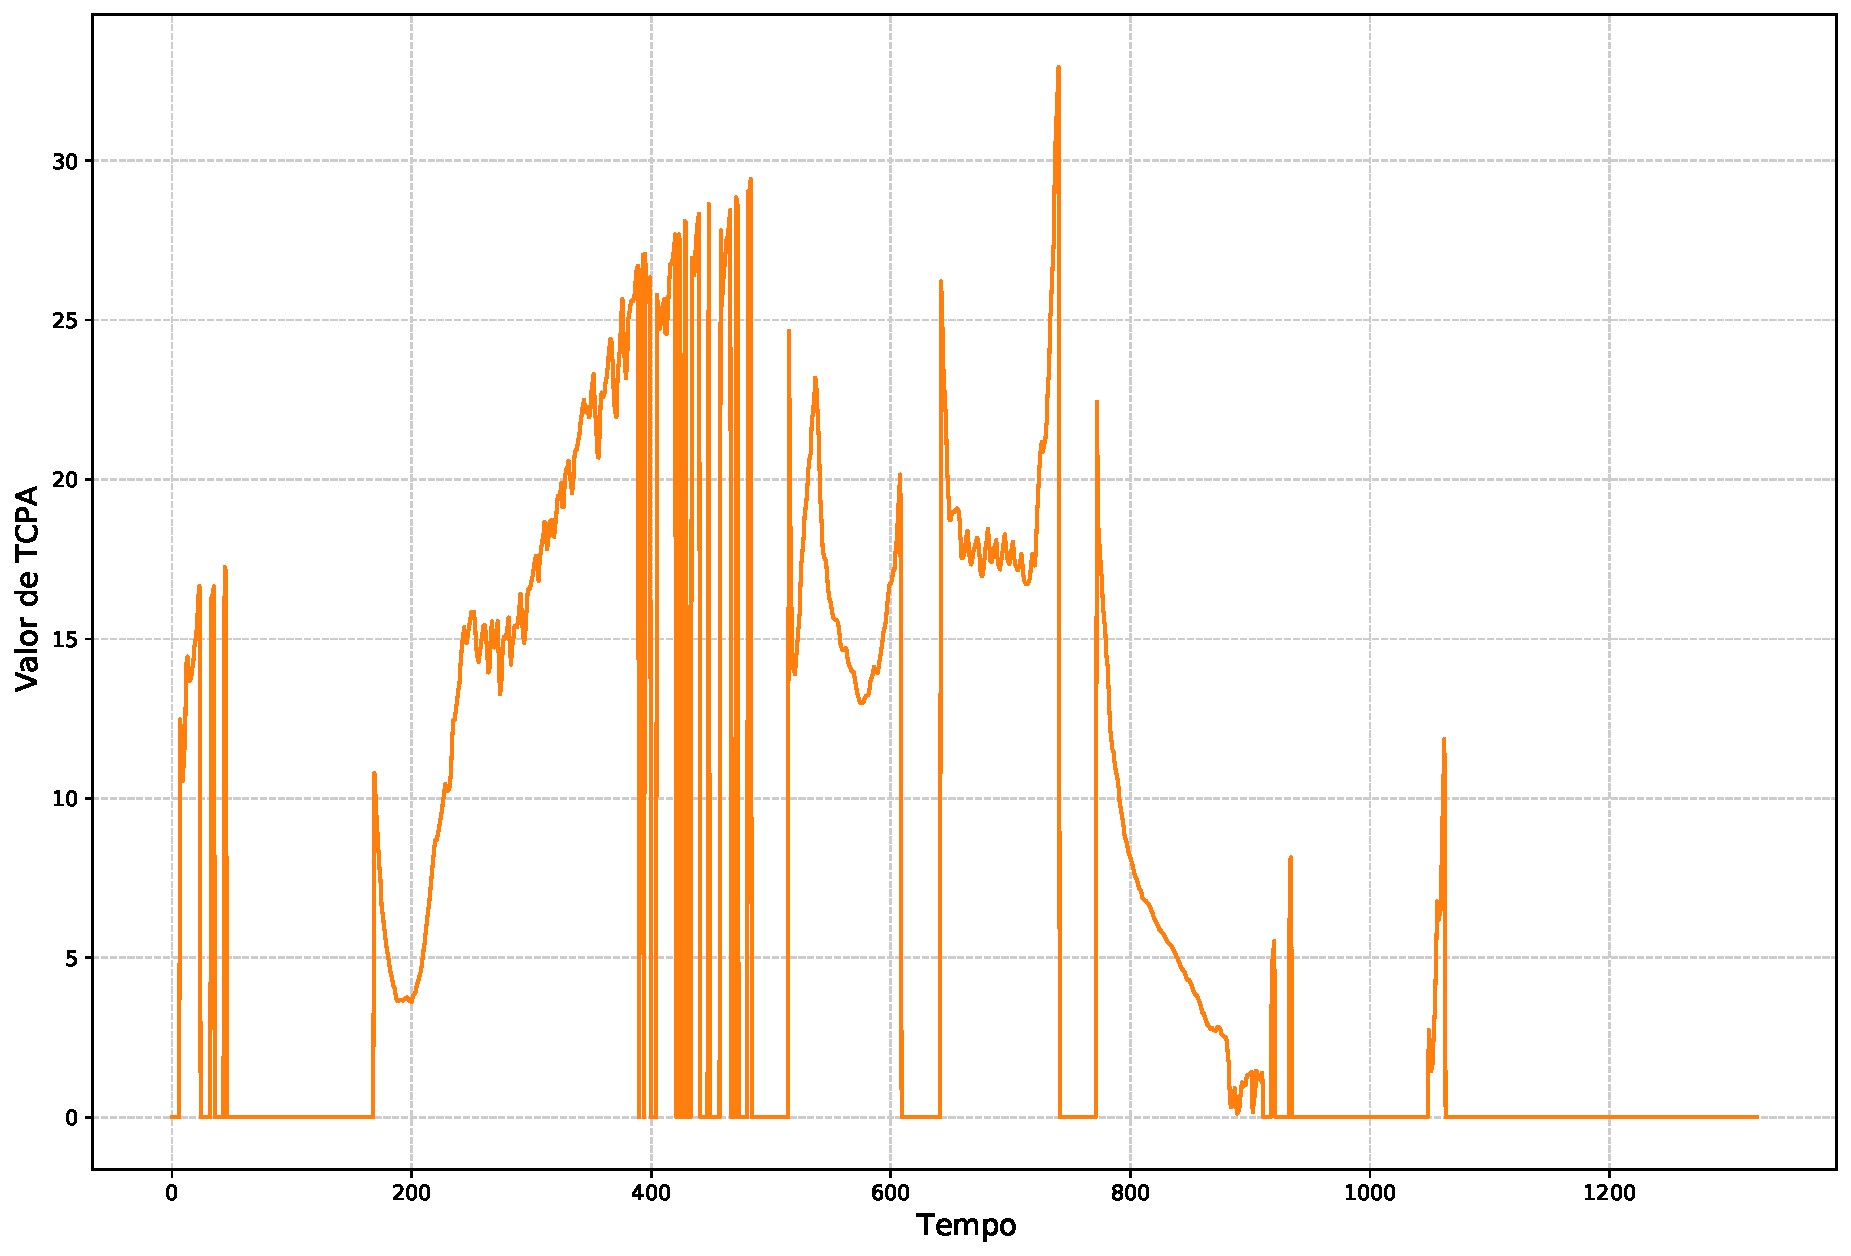
\includegraphics[width=\textwidth]{fig/chap5/crossing_left_tcpa.pdf}
            \caption{TCPA}
            \label{fig:chap5_crossing_left_tcpa}
        \end{subfigure}
        % \begin{subfigure}{0.5\textwidth}
        \begin{subfigure}{1\textwidth}
            \centering
            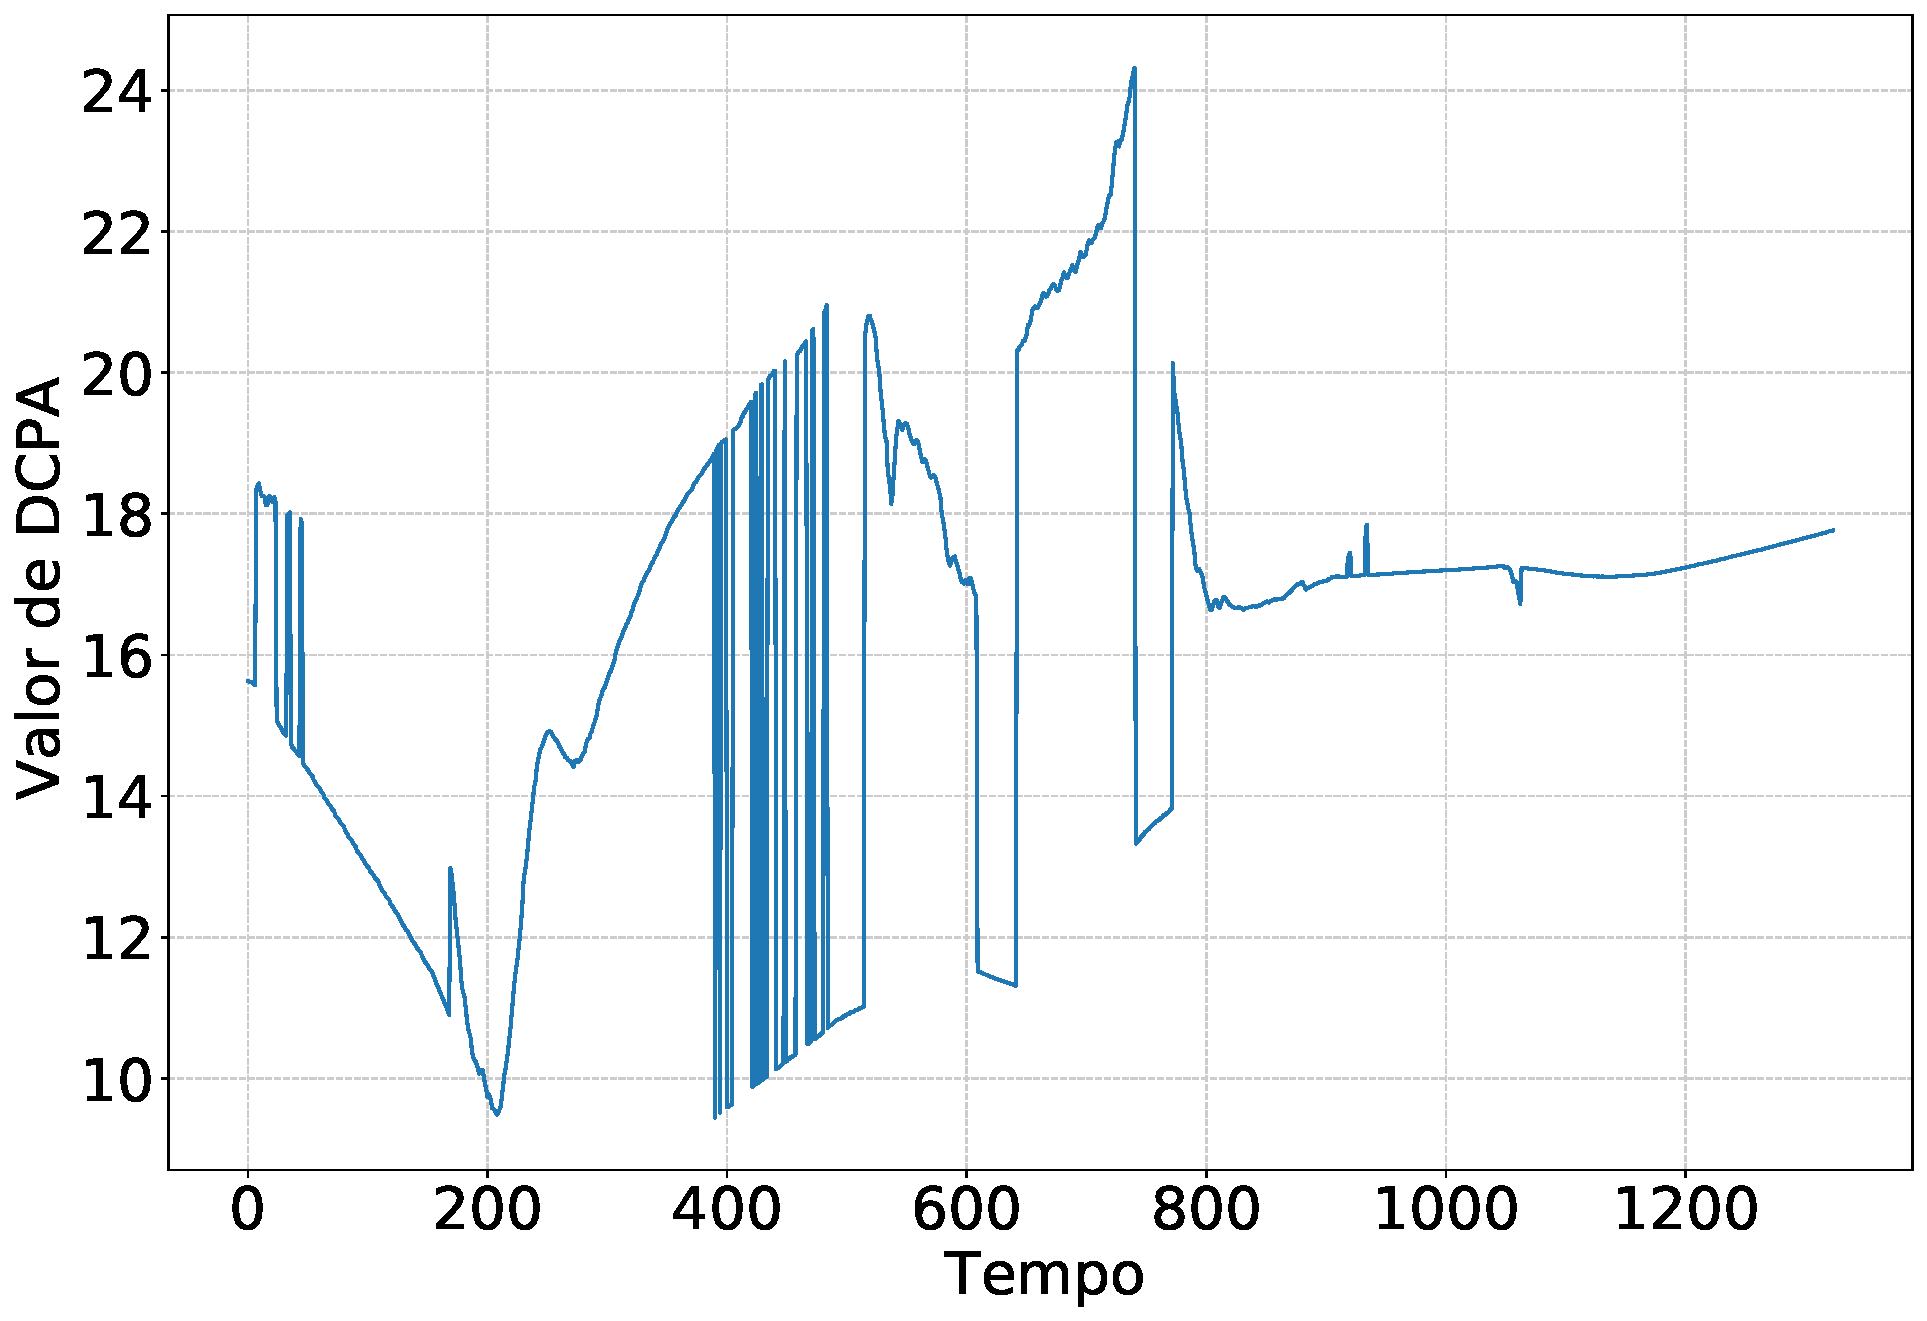
\includegraphics[width=\textwidth]{fig/chap5/crossing_left_dcpa.pdf}
            \caption{DCPA}
            \label{fig:chap5_crossing_left_dcpa}
        \end{subfigure}
        
        \caption{Informações do CPA}
        \label{fig:chap5_crossing_left_cpa}
        \end{figure}
        
        \begin{figure}[H]
            \centering
            % 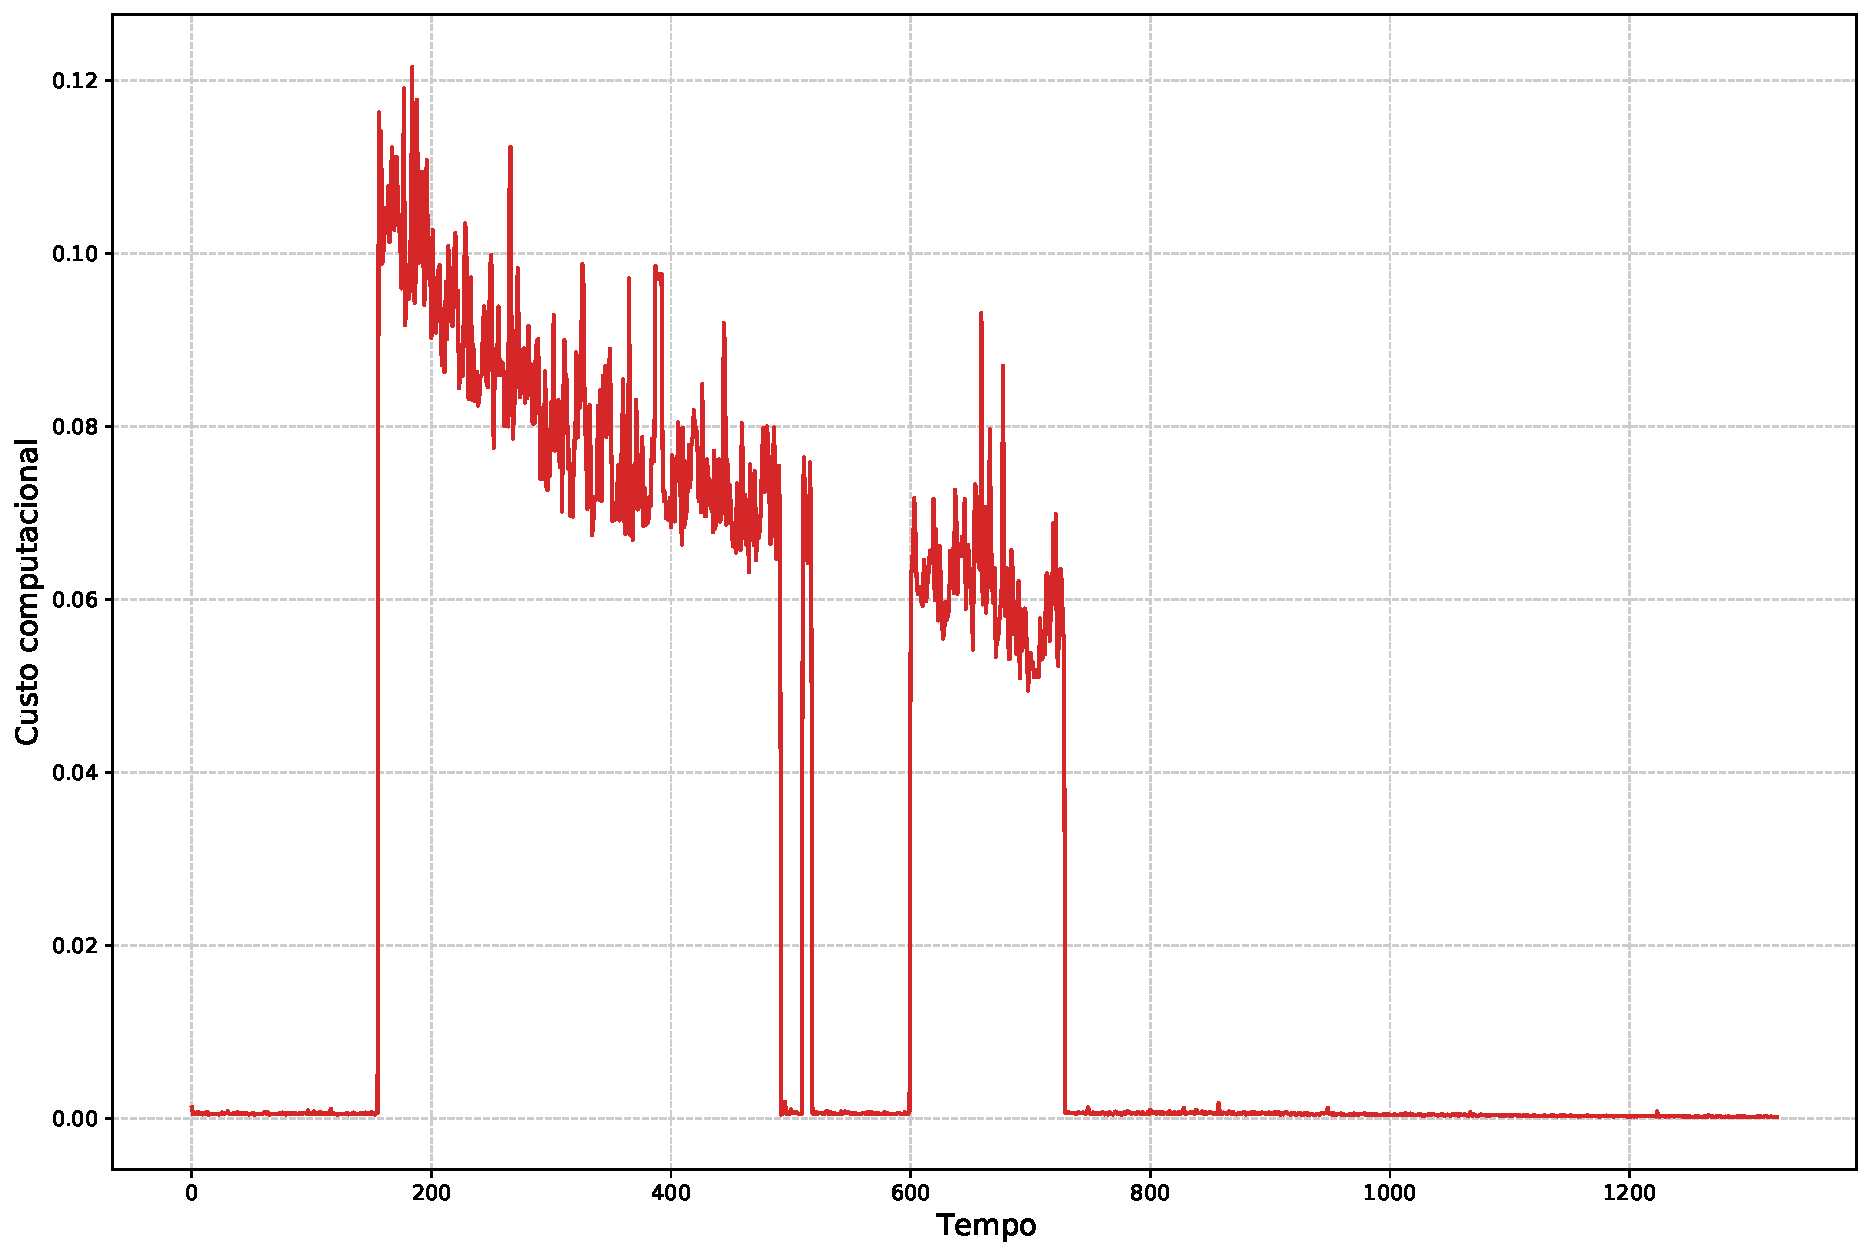
\includegraphics[scale=0.3]{fig/chap5/crossing_left_computation_time.pdf}
            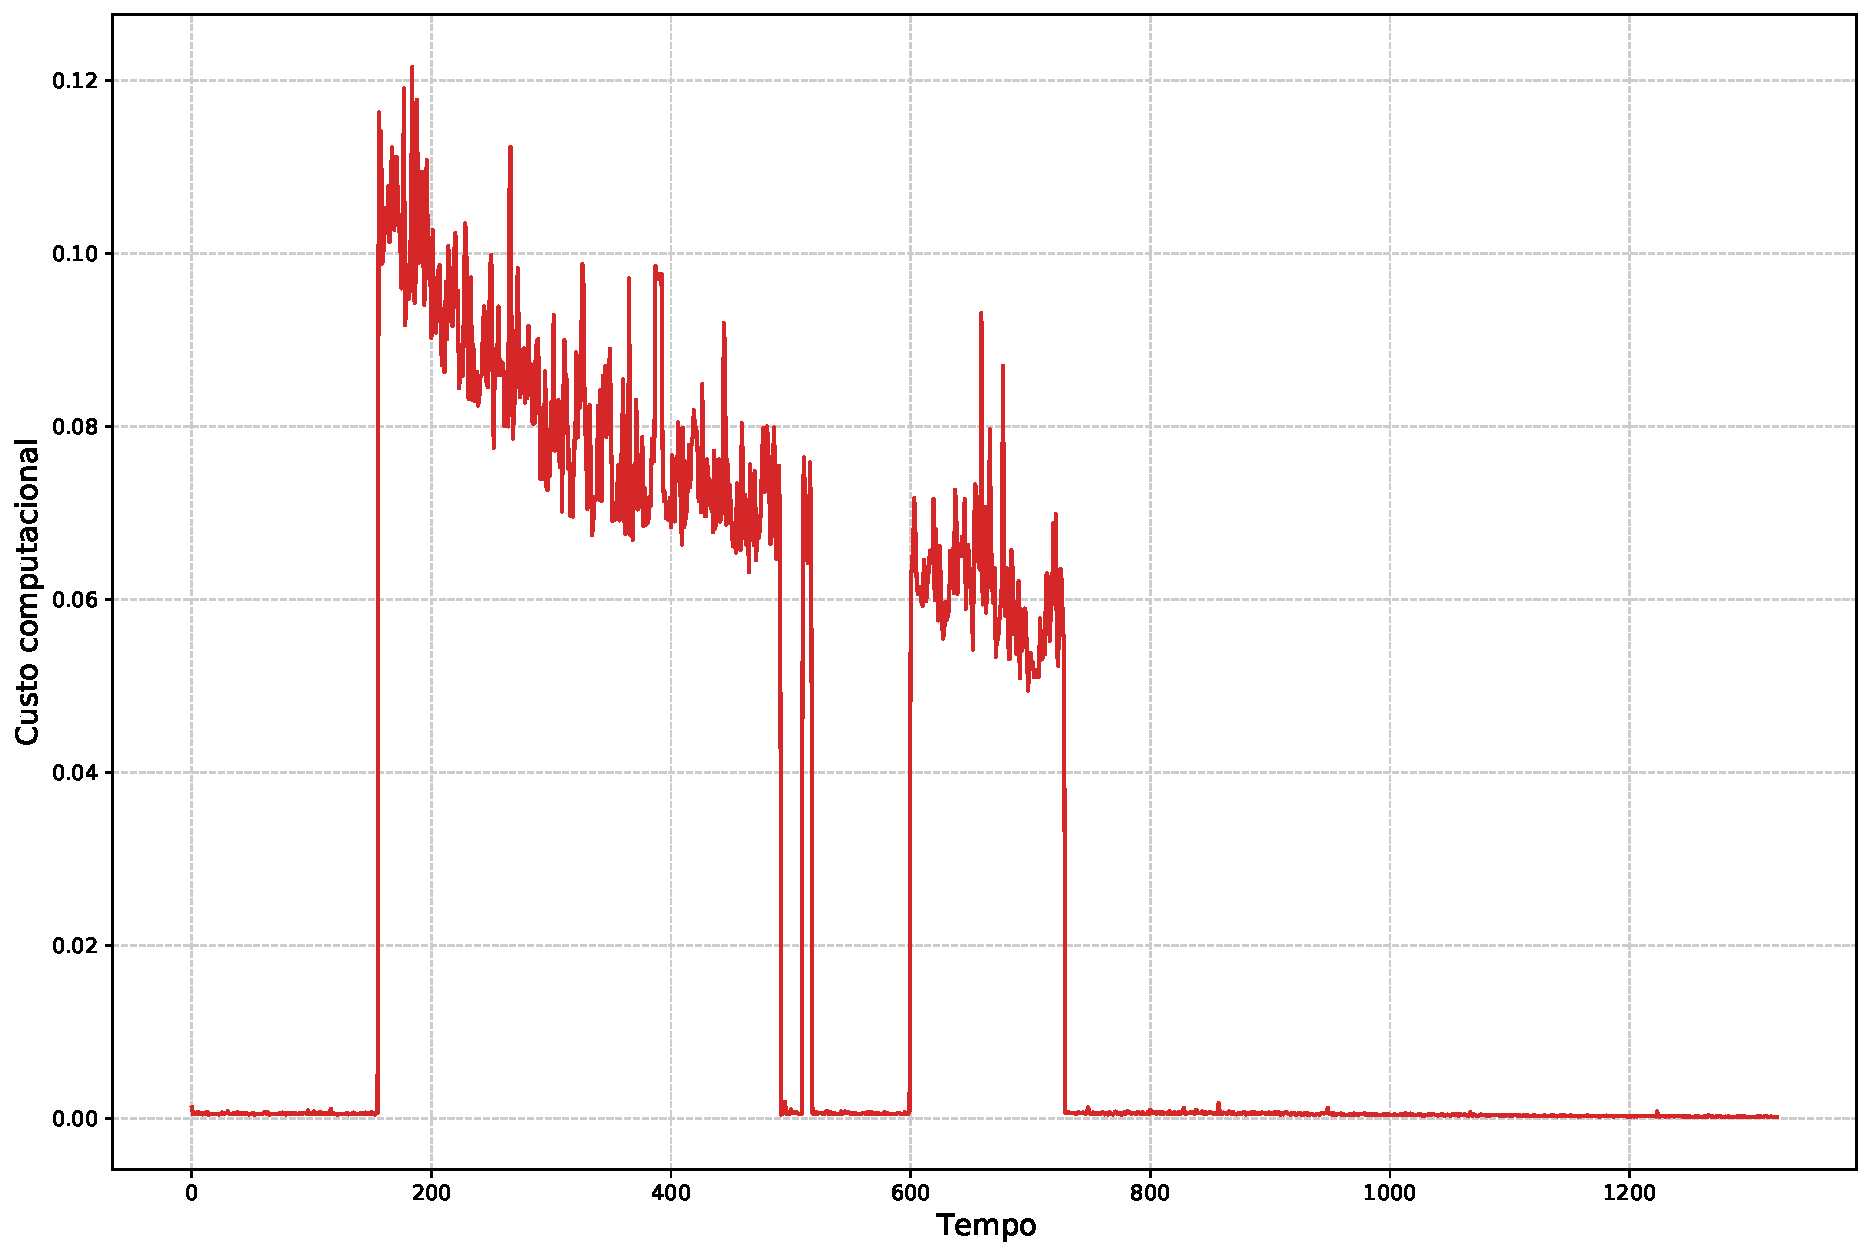
\includegraphics[width=\textwidth]{fig/chap5/crossing_left_computation_time.pdf}
            \caption{Tempo de computação}
            \label{fig:chap5_crossing_left_computation_time}
        \end{figure}
        
    \section{Crossing from Right} \label{subchap5_crossing_from_right}
        A Figura~\ref{fig:chap5_crossing_right_paths} apresenta a trajetória das embarcações para o presente caso de teste, onde o USV encontra a outra embarcação vindo pelo seu lado direito. Nesse caso o USV é responsável por evitar uma possível colisão, desviando de sua rota original pela direita a fim de passar por trás da outra embarcação. Novamente a linha azul representa o trajeto realizado pelo USV enquanto que a linha vermelha representa o trajeto da outra 
        embarcação. A menor distância registrada nesse teste foi de 1,866m e a posição das embarcações nesse momento está indicada pelos triângulos em cada linha na imagem. A análise do \tcpa e do \dcpa, ilustrados respectivamente pela Figura~\ref{fig:chap5_crossing_right_tcpa} e Figura~\ref{fig:chap5_crossing_right_dcpa}, são análogas às análises anteriores. Ou seja, conforme as embarcações vão se aproximando menor é o \tcpa e \dcpa calculado, conforme a distância entre as embarcações vai aumentando a tendência é que o \tcpa e o \dcpa também aumentem em decorrência da distância. O tempo de computação, ilustrado pela Figura~\ref{fig:chap5_crossing_right_computation_time}, tem seus picos justificados pelo planejamento necessário enquanto a outra embarcação estiver no alcance do planejador local.
    
        \begin{figure}[H]
            \centering
            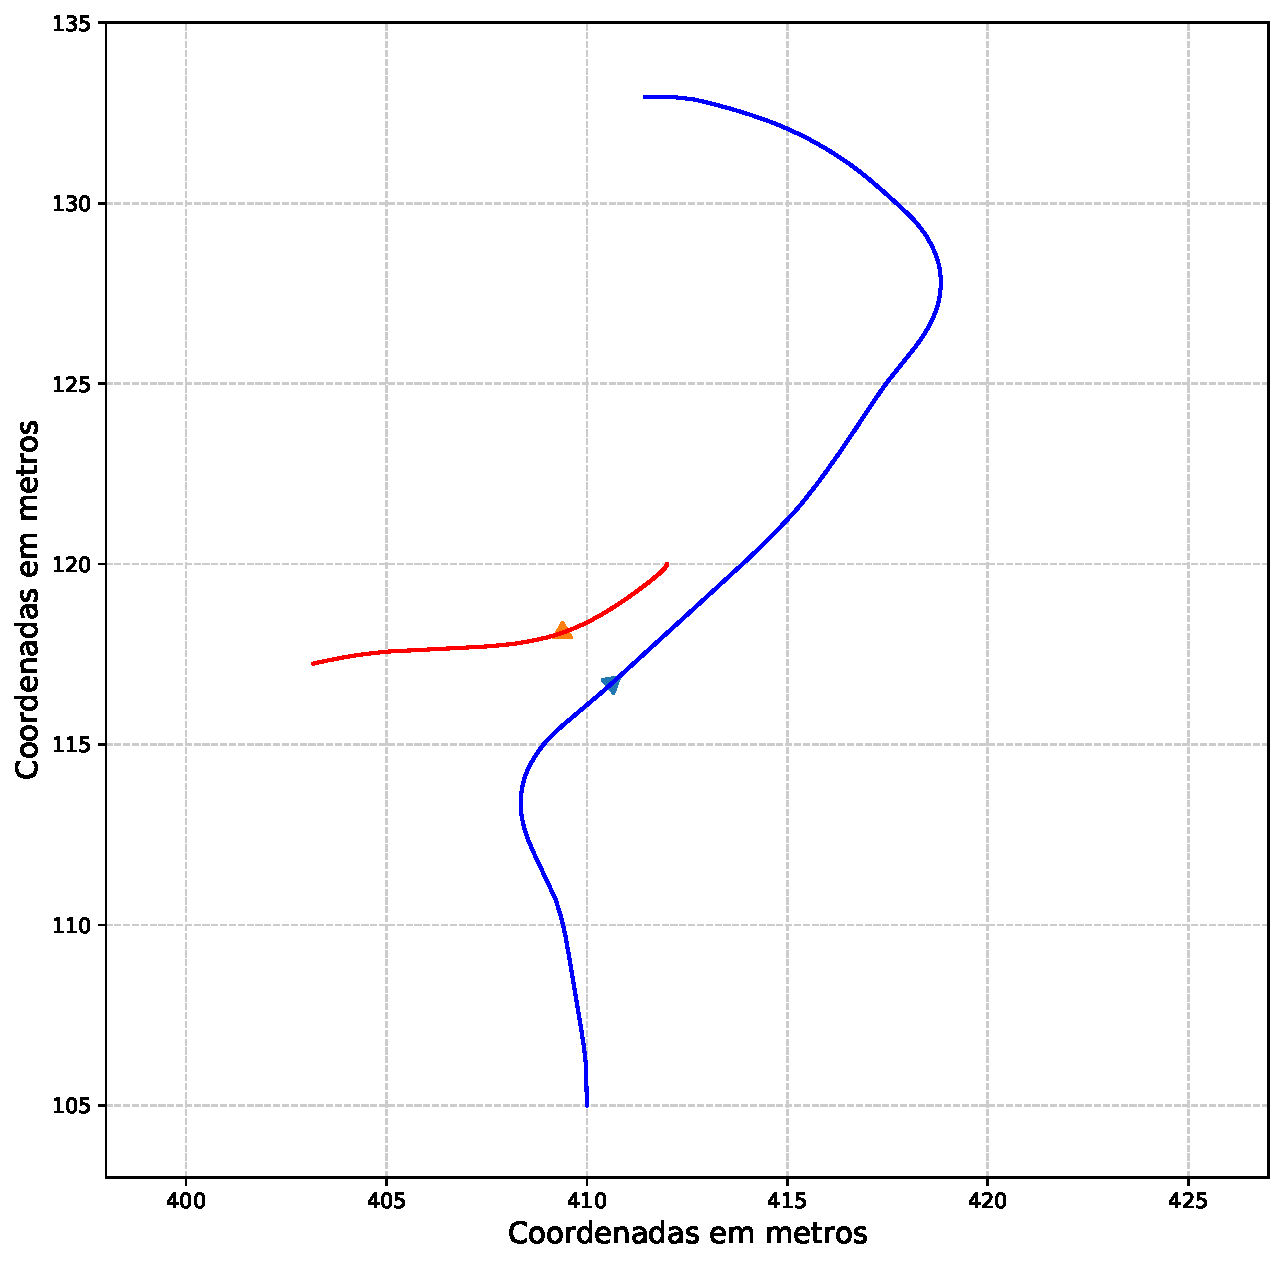
\includegraphics[scale=0.45]{fig/chap5/crossing_right_trajectory.pdf}
            \caption{Trajeto das embarcações}
            \label{fig:chap5_crossing_right_paths}
        \end{figure}
        
        \begin{figure}[H]
		\centering
% 		\begin{subfigure}{0.5\textwidth}
		\begin{subfigure}{1\textwidth}
            \centering
            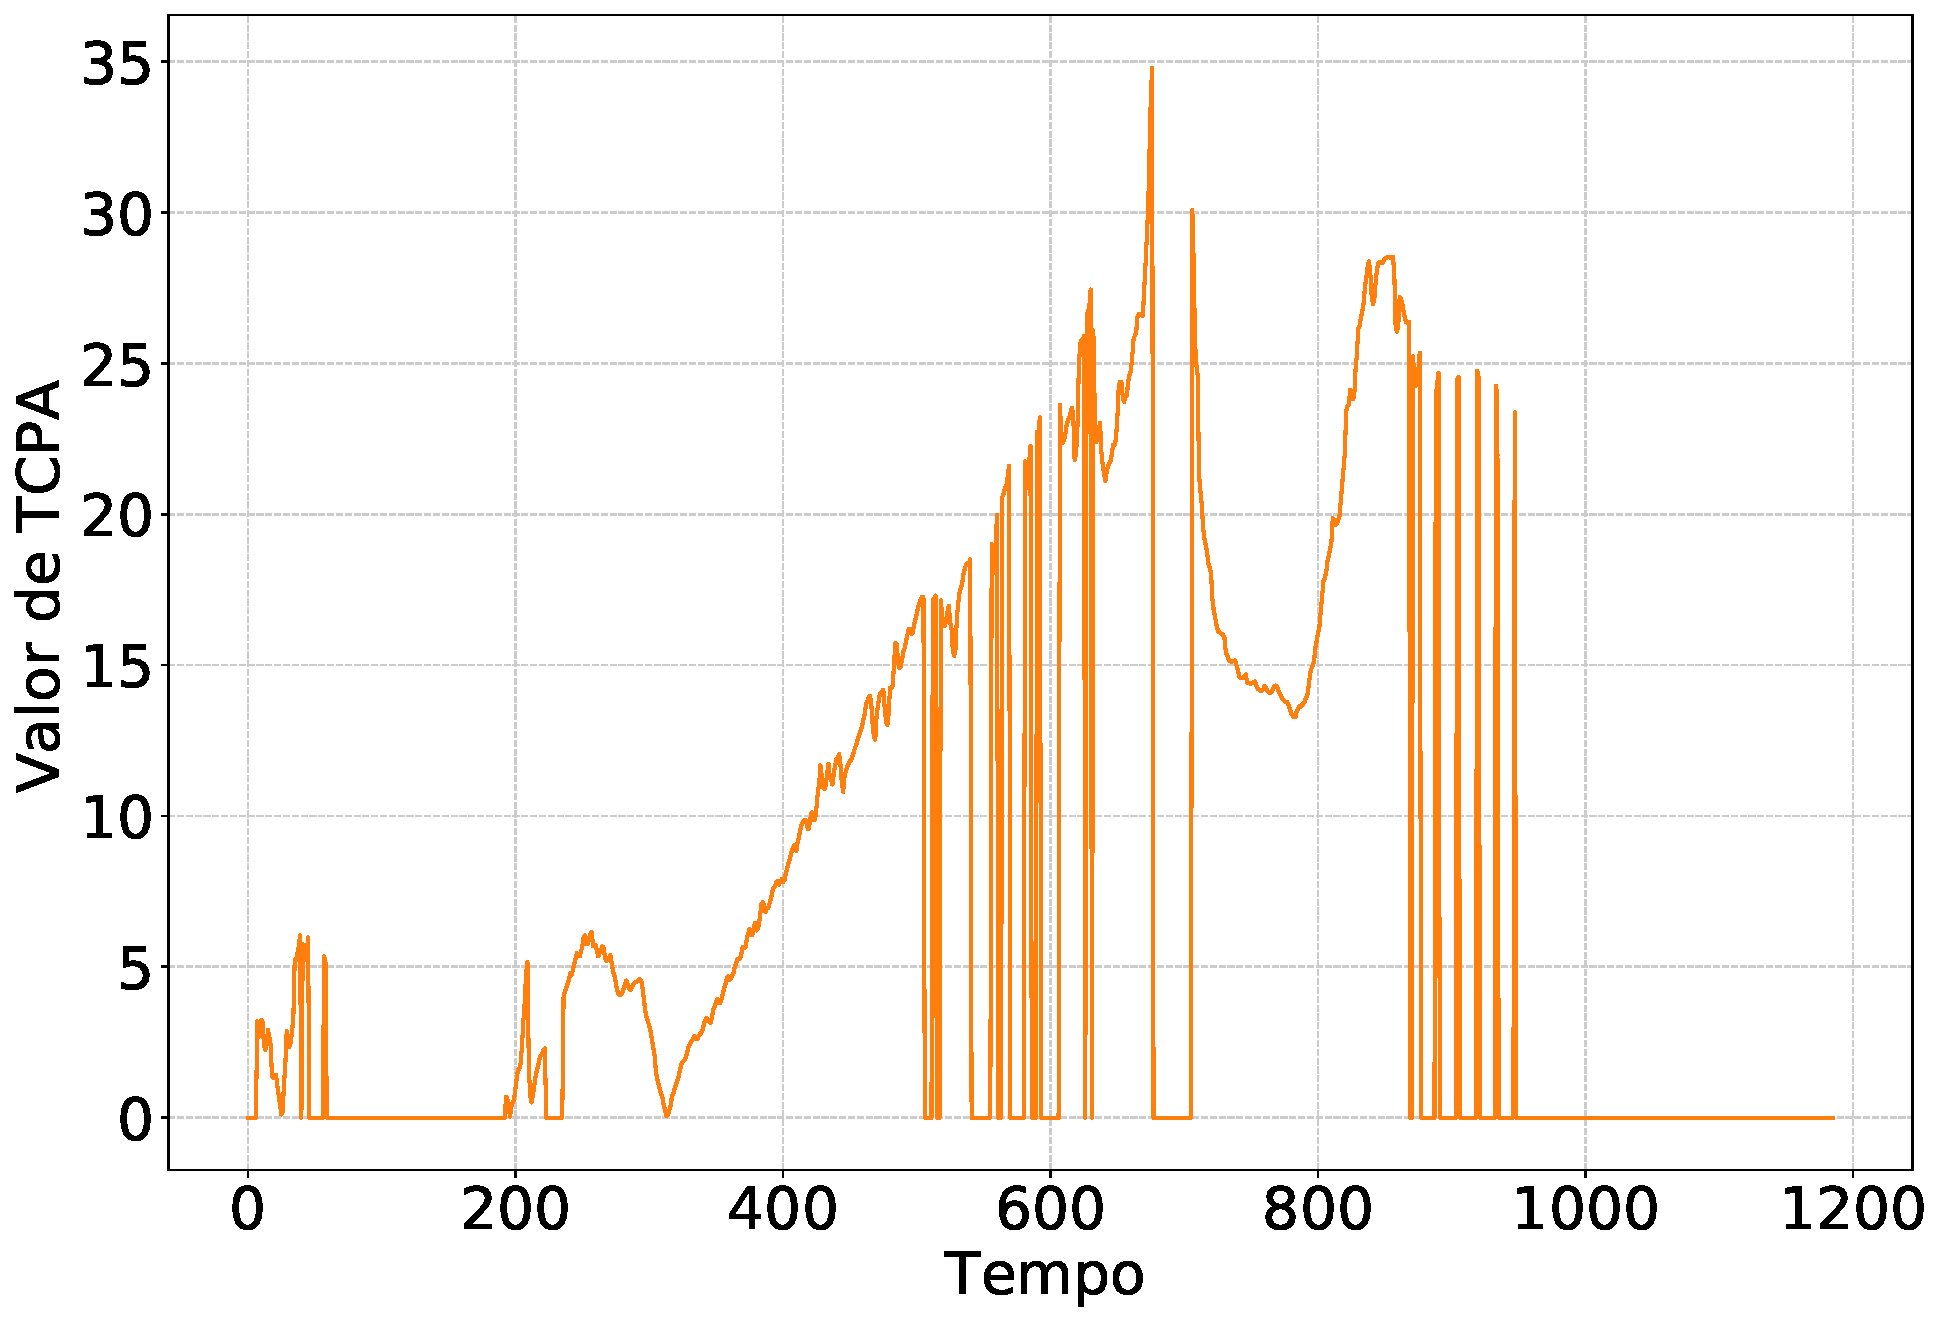
\includegraphics[width=\textwidth]{fig/chap5/crossing_right_tcpa.pdf}
            \caption{TCPA}
            \label{fig:chap5_crossing_right_tcpa}
        \end{subfigure}
        % \begin{subfigure}{0.5\textwidth}
        \begin{subfigure}{1\textwidth}
            \centering
            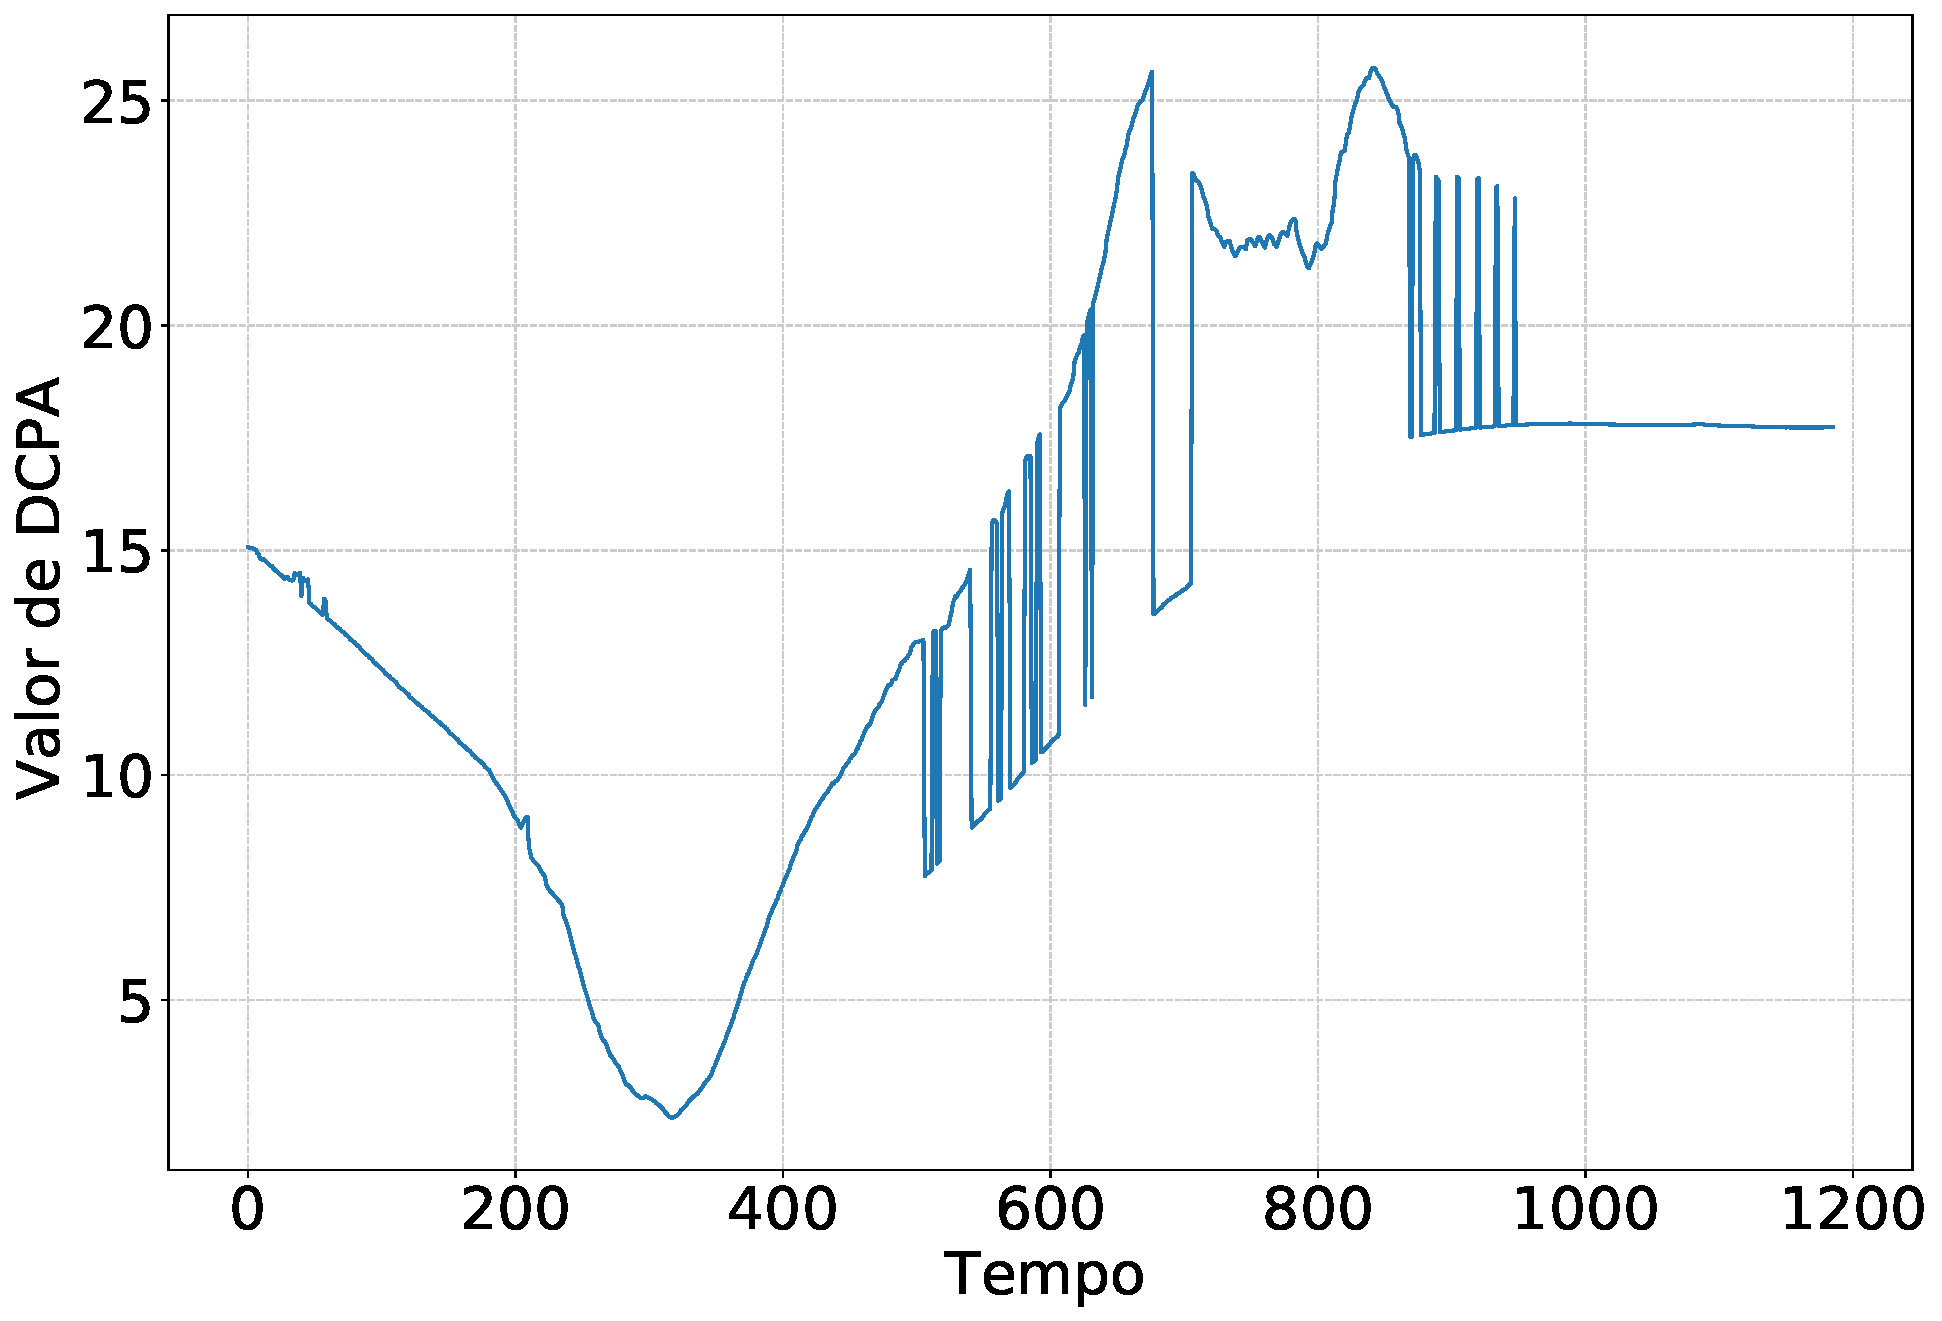
\includegraphics[width=\textwidth]{fig/chap5/crossing_right_dcpa.pdf}
            \caption{DCPA}
            \label{fig:chap5_crossing_right_dcpa}
        \end{subfigure}
        
        \caption{Informações do CPA}
        \label{fig:chap5_crossing_right_cpa}
        \end{figure}
        
        \begin{figure}[H]
            \centering
            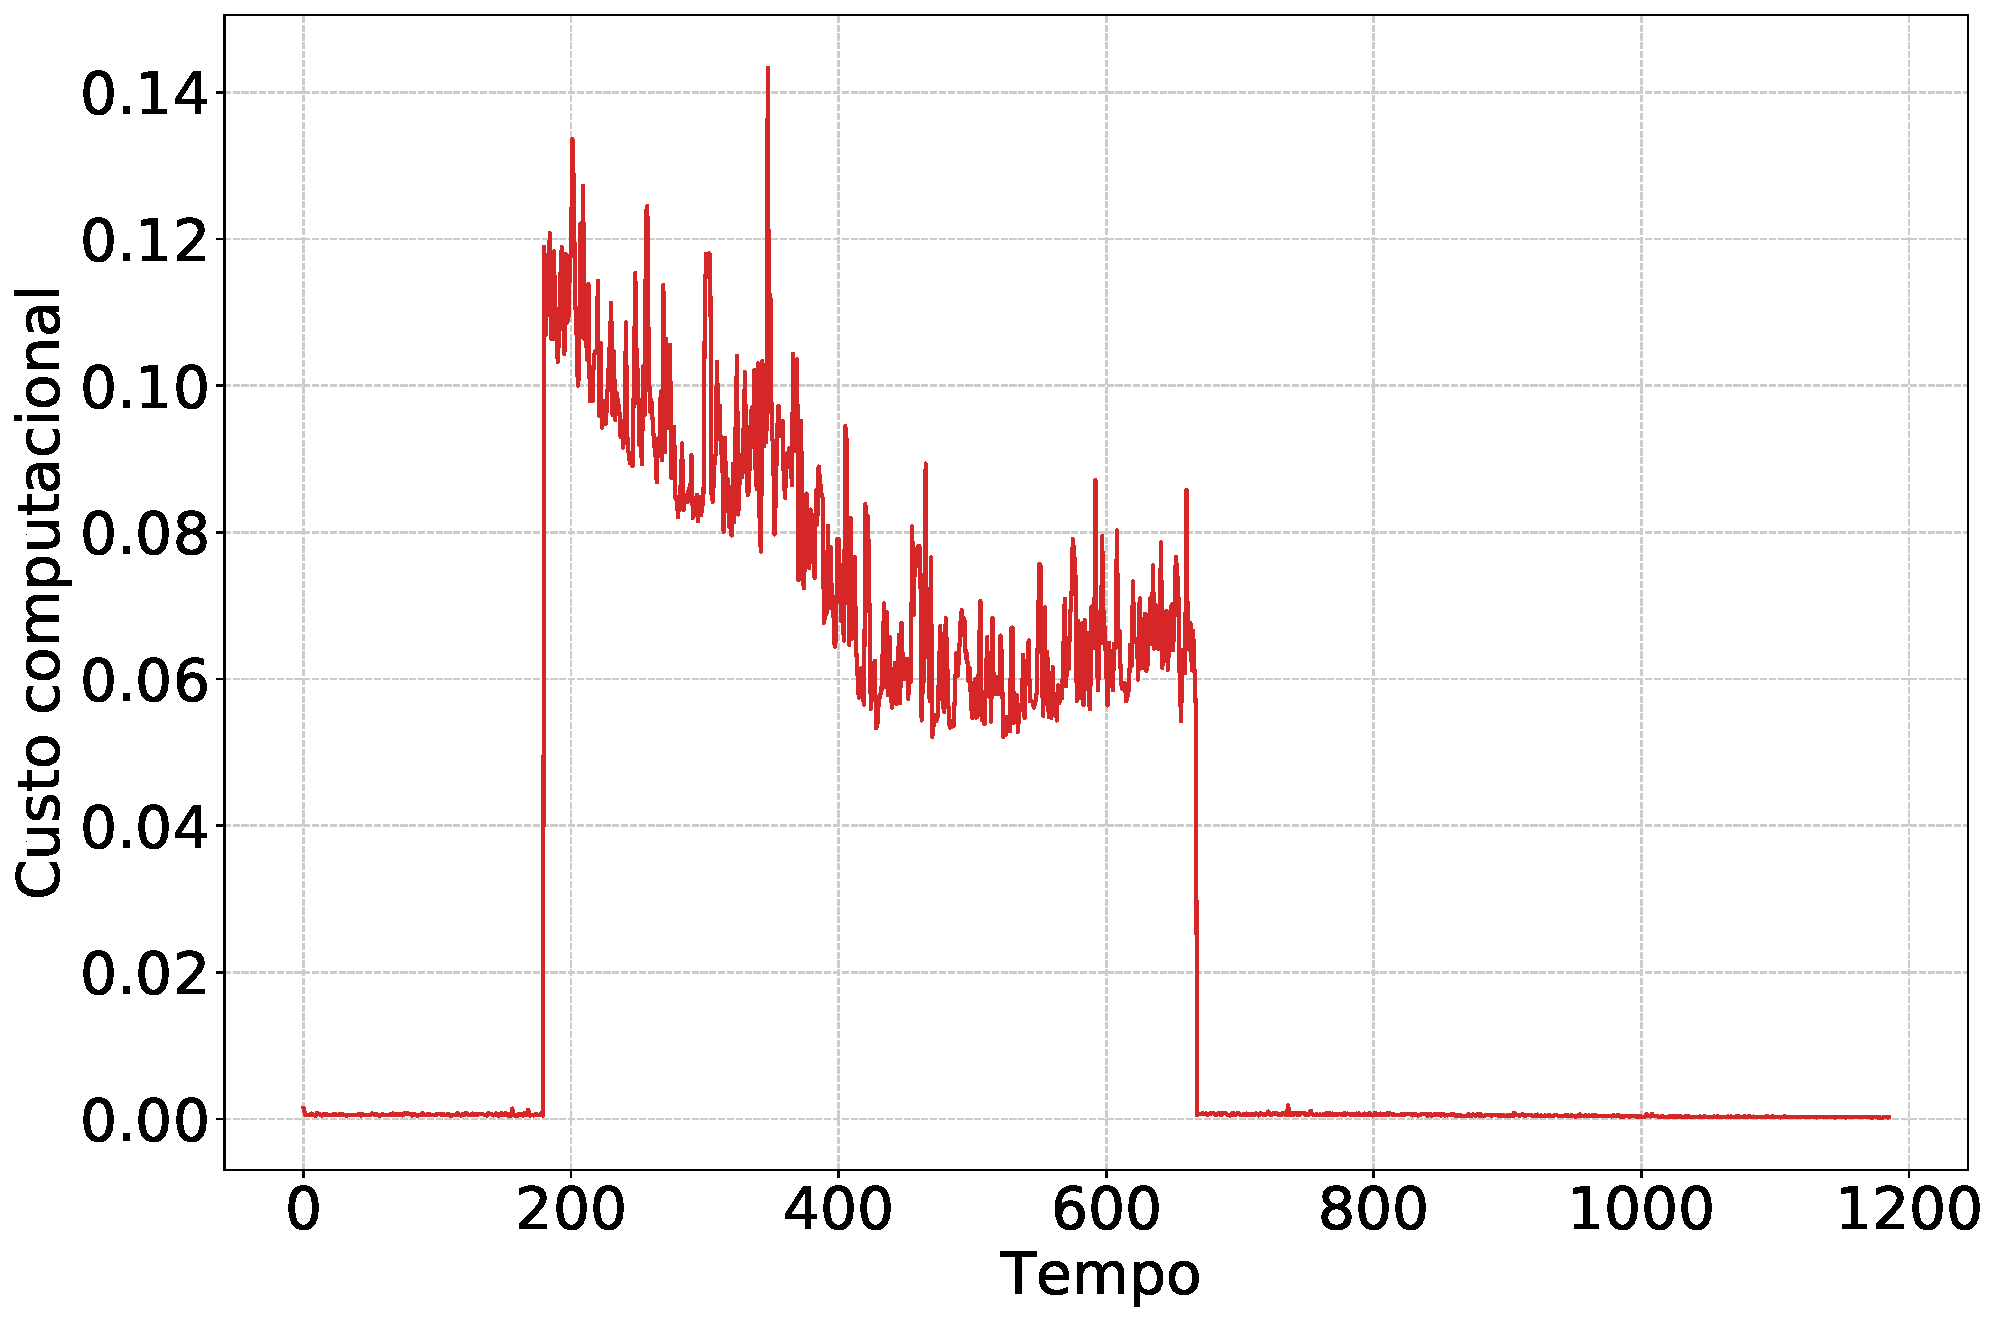
\includegraphics[width=\textwidth]{fig/chap5/crossing_right_computation_time.pdf}
            \caption{Tempo de computação}
            \label{fig:chap5_crossing_right_computation_time}
        \end{figure}
        
    \section{Crossing from Right - Embarcação Parada}
        Nessa seção apresentaremos os casos de teste onde nossa implementação se torna evidente. Realizamos novamente o caso de teste \textit{"Crossing from Right"} porém agora a outra embarcação ficará parada durante todo o teste. Esse cenário foi executado com duas configurações diferentes no sistema base: sem CPA e com CPA.
    
        \subsection{Sem CPA}
            Primeiramente apresentaremos os resultados obtidos ao executar o cenário \textit{"Crossing from Right"} com a outra embarcação parada e sem a implementação do CPA no sistema base do USV. A Figura~\ref{fig:chap5_crossing_right_stopped_vessel_no_cpa_paths} mostra o trajeto realizado pelo USV. Como pode-se observar, mesmo com a outra embarcação parada o USV tenta realizar uma manobra em conformidade com as COLREGS. Da imagem apresentada também é possível inferir que o USV não obteve sucesso na tentativa de passar por trás da outra embarcação, como requisitado pela COLREGS. Nesse caso, a distância mínima registrada durante o encontro foi de 1,352m. A Figura~\ref{fig:chap5_crossing_right_stopped_vessel_no_cpa_computation_time} mostra o tempo de computação necessário para executar a rotina apresentada no Capítulo~\ref{chap4:desenvolvimento}. Nesse caso, é possível observar um elevado esforço computacional durante quase todo o percurso, ocasionado pela criação dos obstáculos virtuais e a necessidade de planejar uma rota local. Após passar pela outra embarcação e começar a se afastar o esforço necessário diminui, dado que não é mais preciso contornar o obstáculo.
    
            \begin{figure}[H]
                \centering
                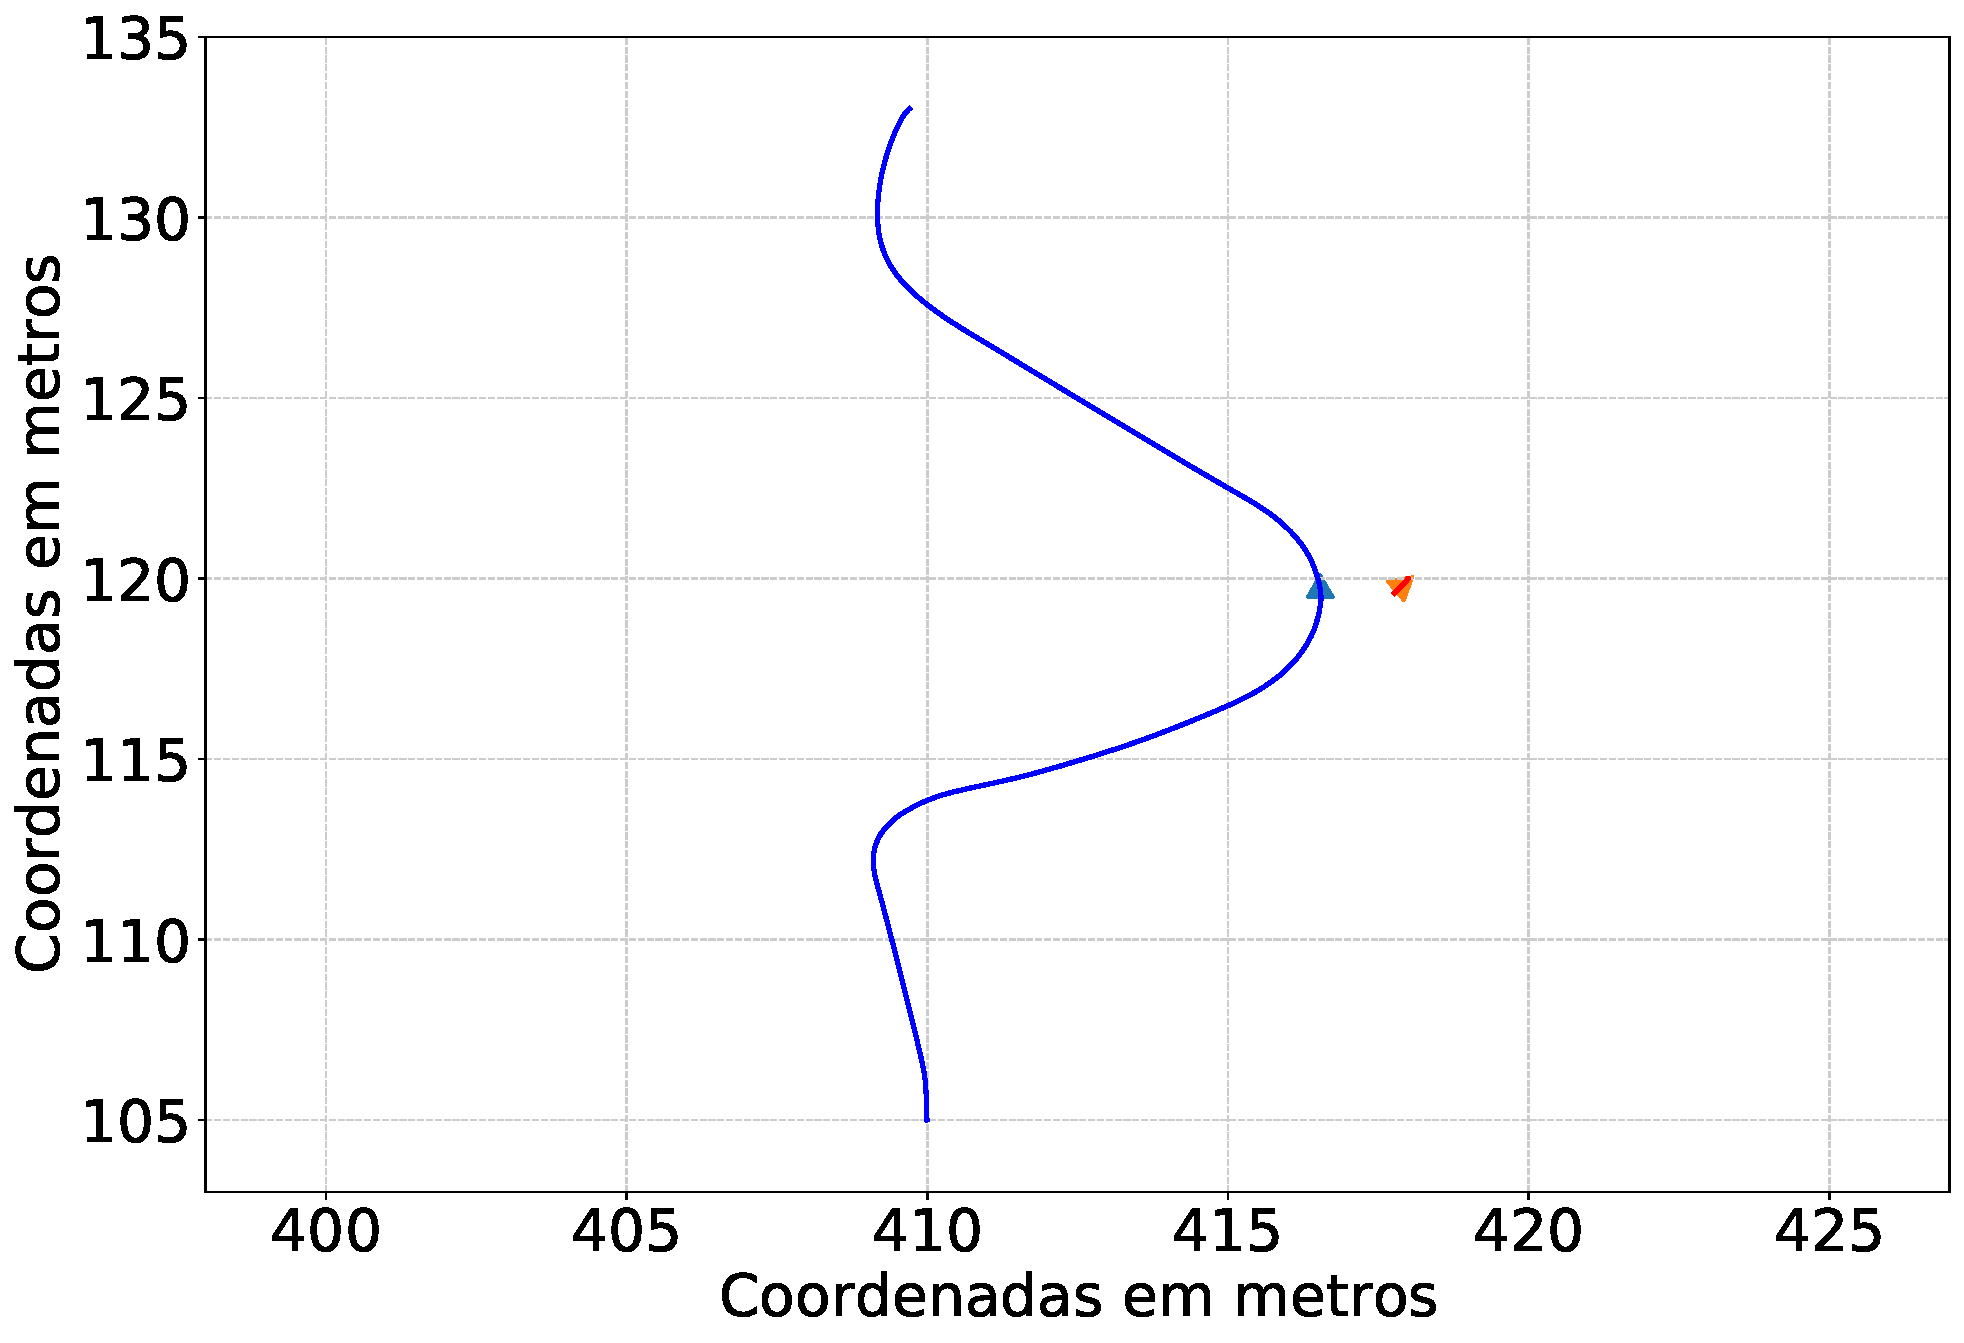
\includegraphics[scale=0.45]{fig/chap5/crossing_right_stopped_vessel_no_cpa_trajectory.pdf}
                \caption{Trajeto das embarcações}
                \label{fig:chap5_crossing_right_stopped_vessel_no_cpa_paths}
            \end{figure}
            
            \begin{figure}[H]
                \centering
                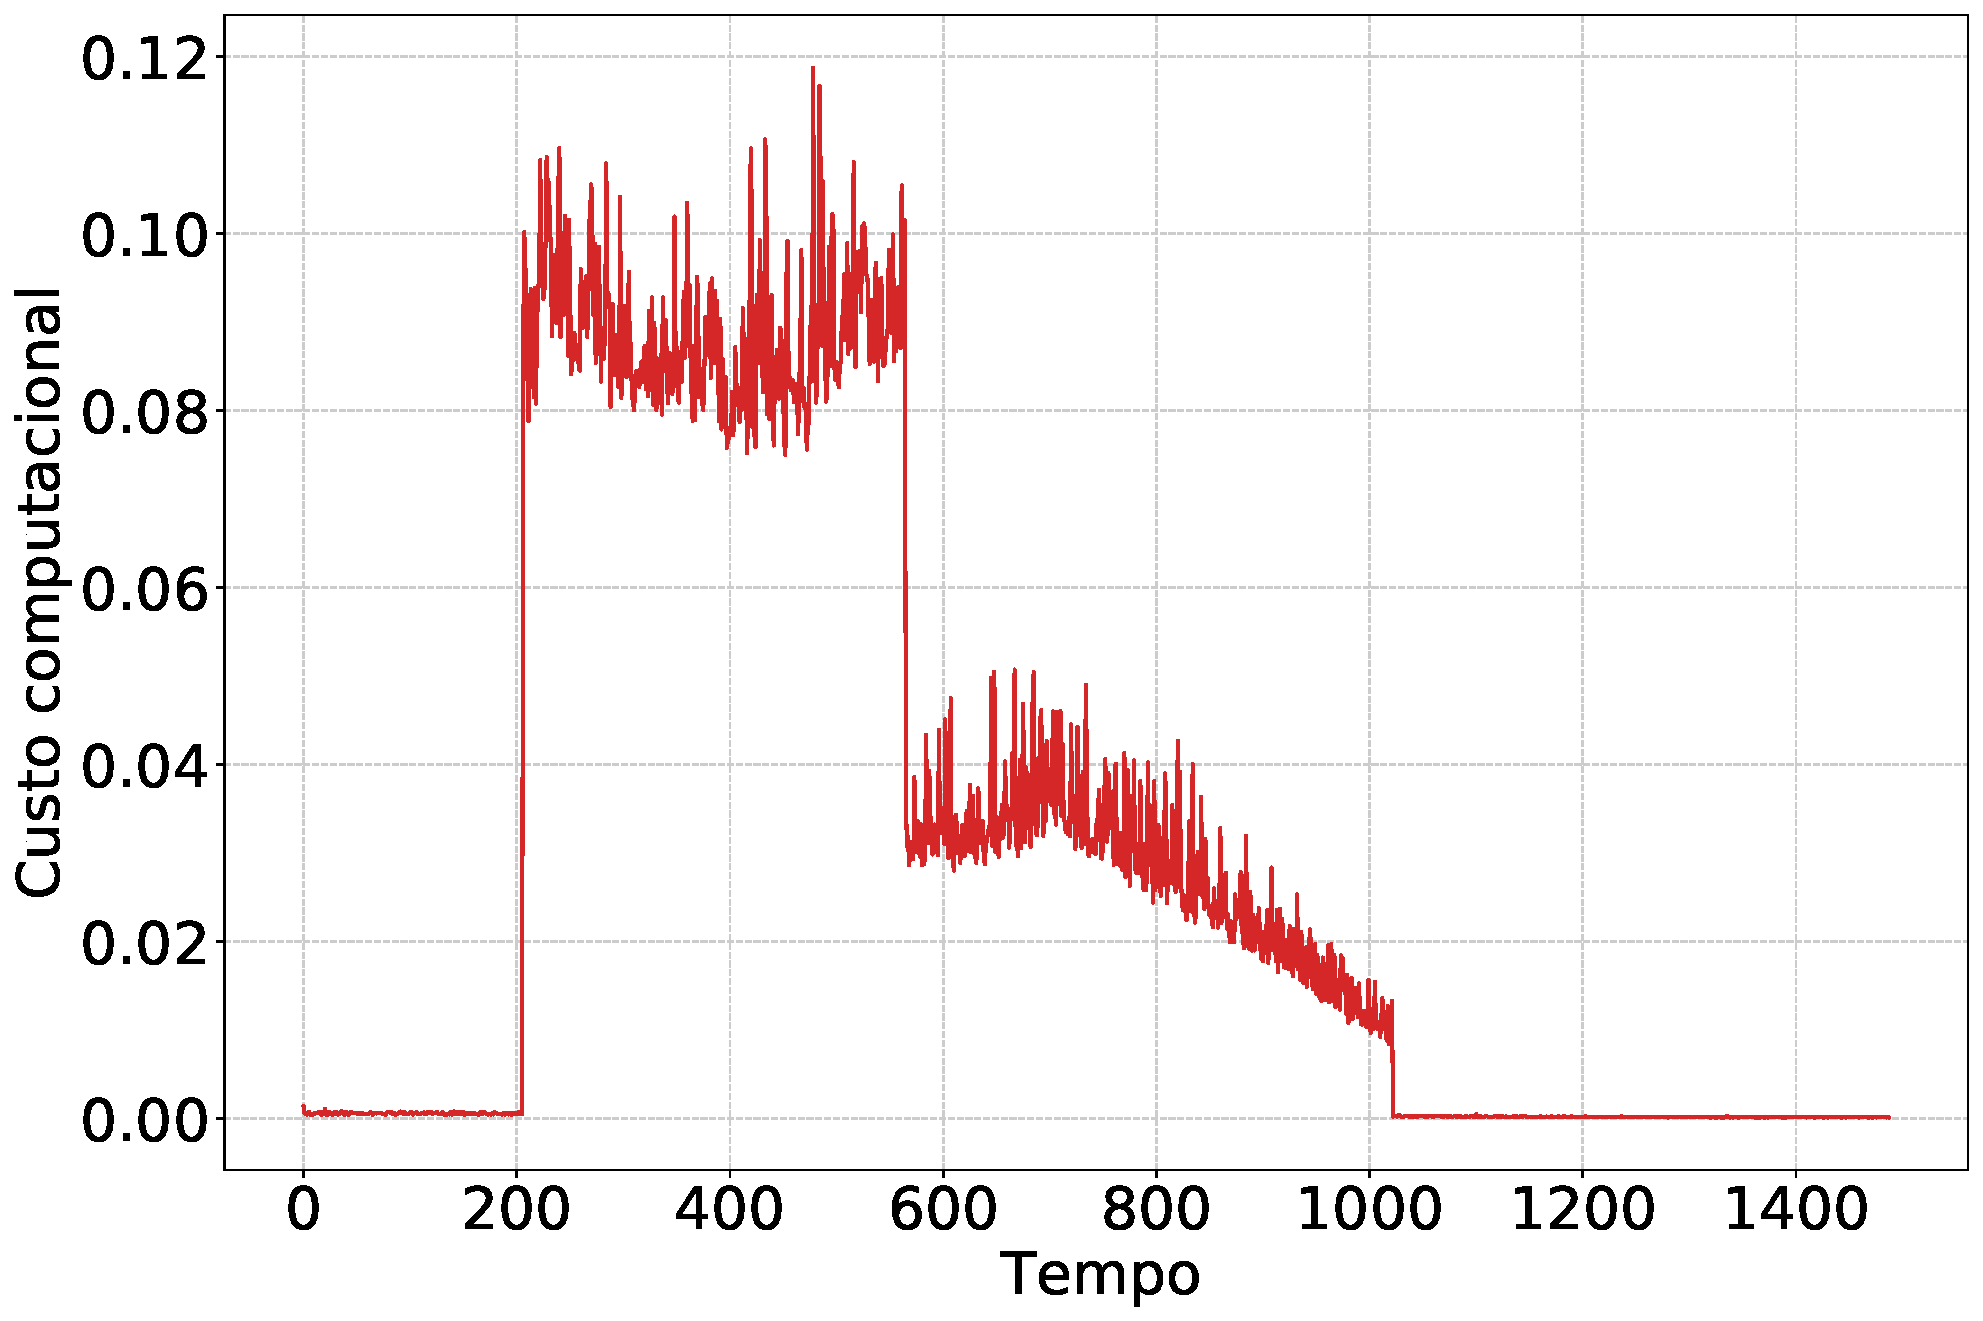
\includegraphics[scale=0.3]{fig/chap5/crossing_right_stopped_vessel_no_cpa_computation_time.pdf}
                \caption{Tempo de computação}
                \label{fig:chap5_crossing_right_stopped_vessel_no_cpa_computation_time}
            \end{figure}
            
        \subsection{Com CPA}\label{subsection_crossing_right_stopped_vessel_cpa}
            Executando o mesmo caso de teste com o CPA integrado no sistema do USV podemos observar, na Figura~\ref{fig:chap5_crossing_right_stopped_vessel_cpa_paths}, que obtivemos um resultado diferente. Novamente, a linha azul indica a rota realizada pelo USV enquanto que o triângulo vermelho indica a posição que a outra embarcação ficou durante todo o teste. O triângulo azul indica a posição do USV no momento em que a menor distância entre as embarcações foi registrada, que nesse caso foi de 10,443m. Analisando a Figura~\ref{fig:chap5_crossing_right_stopped_vessel_cpa_paths} isoladamente ficamos inclinados a entender que o CPA realizou a função desejada no sistema, indicando que não haveria risco de colisão e permitindo que o sistema realizasse o planejamento da rota local considerando a outra embarcação apenas como um obstáculo estático. Porém ao analisarmos a Figura~\ref{fig:chap5_crossing_right_stopped_vessel_cpa_computation_time} observamos que houveram dois picos de processamento durante a execução do teste. Tais picos indicam que a outra embarcação entrou no alcance do planejador local. Isso ainda não invalida o correto funcionamento do CPA, porém ao analisarmos a Figura~\ref{fig:chap5_crossing_right_stopped_vessel_cpa_tcpa} e a Figura~\ref{fig:chap5_crossing_right_stopped_vessel_cpa_dcpa}, mais precisamente entre os instantes de tempo 350 e 400, podemos inferir que a Desigualdade~\ref{eq:cpaThreshold} é satisfeita e, portanto, o sistema entende que há risco de colisão e realiza a criação de obstáculos virtuais. Isso causa uma instabilidade no sistema, fazendo com que o planejador local, por alguns instantes de tempo, determine uma rota desnecessária por consequência dos obstáculos virtuais criados. Entretanto, momentos depois o \tcpa e o \dcpa assumem valores que fazem o sistema entender que não há risco de colisão, deixando o planejador local livre para planejar a melhor rota até o objetivo. Isso faz com que o USV se afaste da outra embarcação até que ela saia do alcance do planejador local, dado que esse é um comportamento do planejador. Com a outra embarcação fora de alcance, o planejador local fica livre para determinar a rota mais curta até o objetivo, fazendo com que a outra embarcação entre novamente no alcance do planejador local, ocasionando o segundo pico de computação mostrado na Figura~\ref{fig:chap5_crossing_right_stopped_vessel_cpa_computation_time}.
        
            \begin{figure}[H]
                \centering
                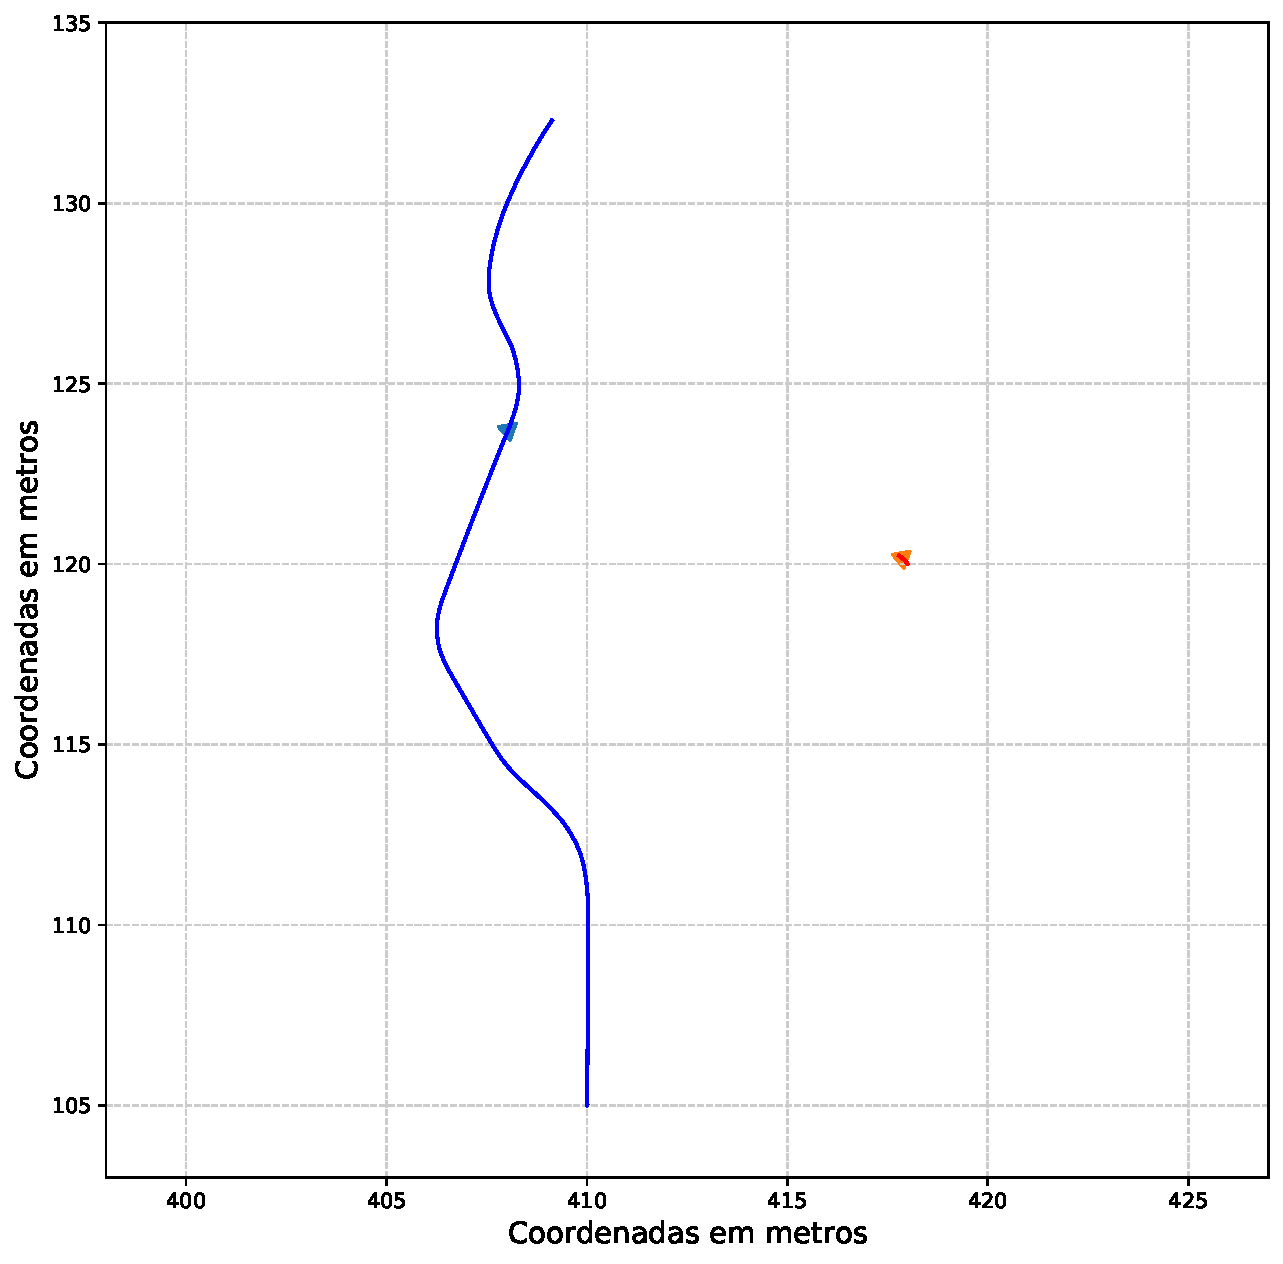
\includegraphics[scale=0.45]{fig/chap5/crossing_right_stopped_vessel_cpa_trajectory.pdf}
                \caption{Trajeto das embarcações}
                \label{fig:chap5_crossing_right_stopped_vessel_cpa_paths}
            \end{figure}
            
            \begin{figure}[H]
    		\centering
    % 		\begin{subfigure}{0.5\textwidth}
            \begin{subfigure}{1\textwidth}
                \centering
                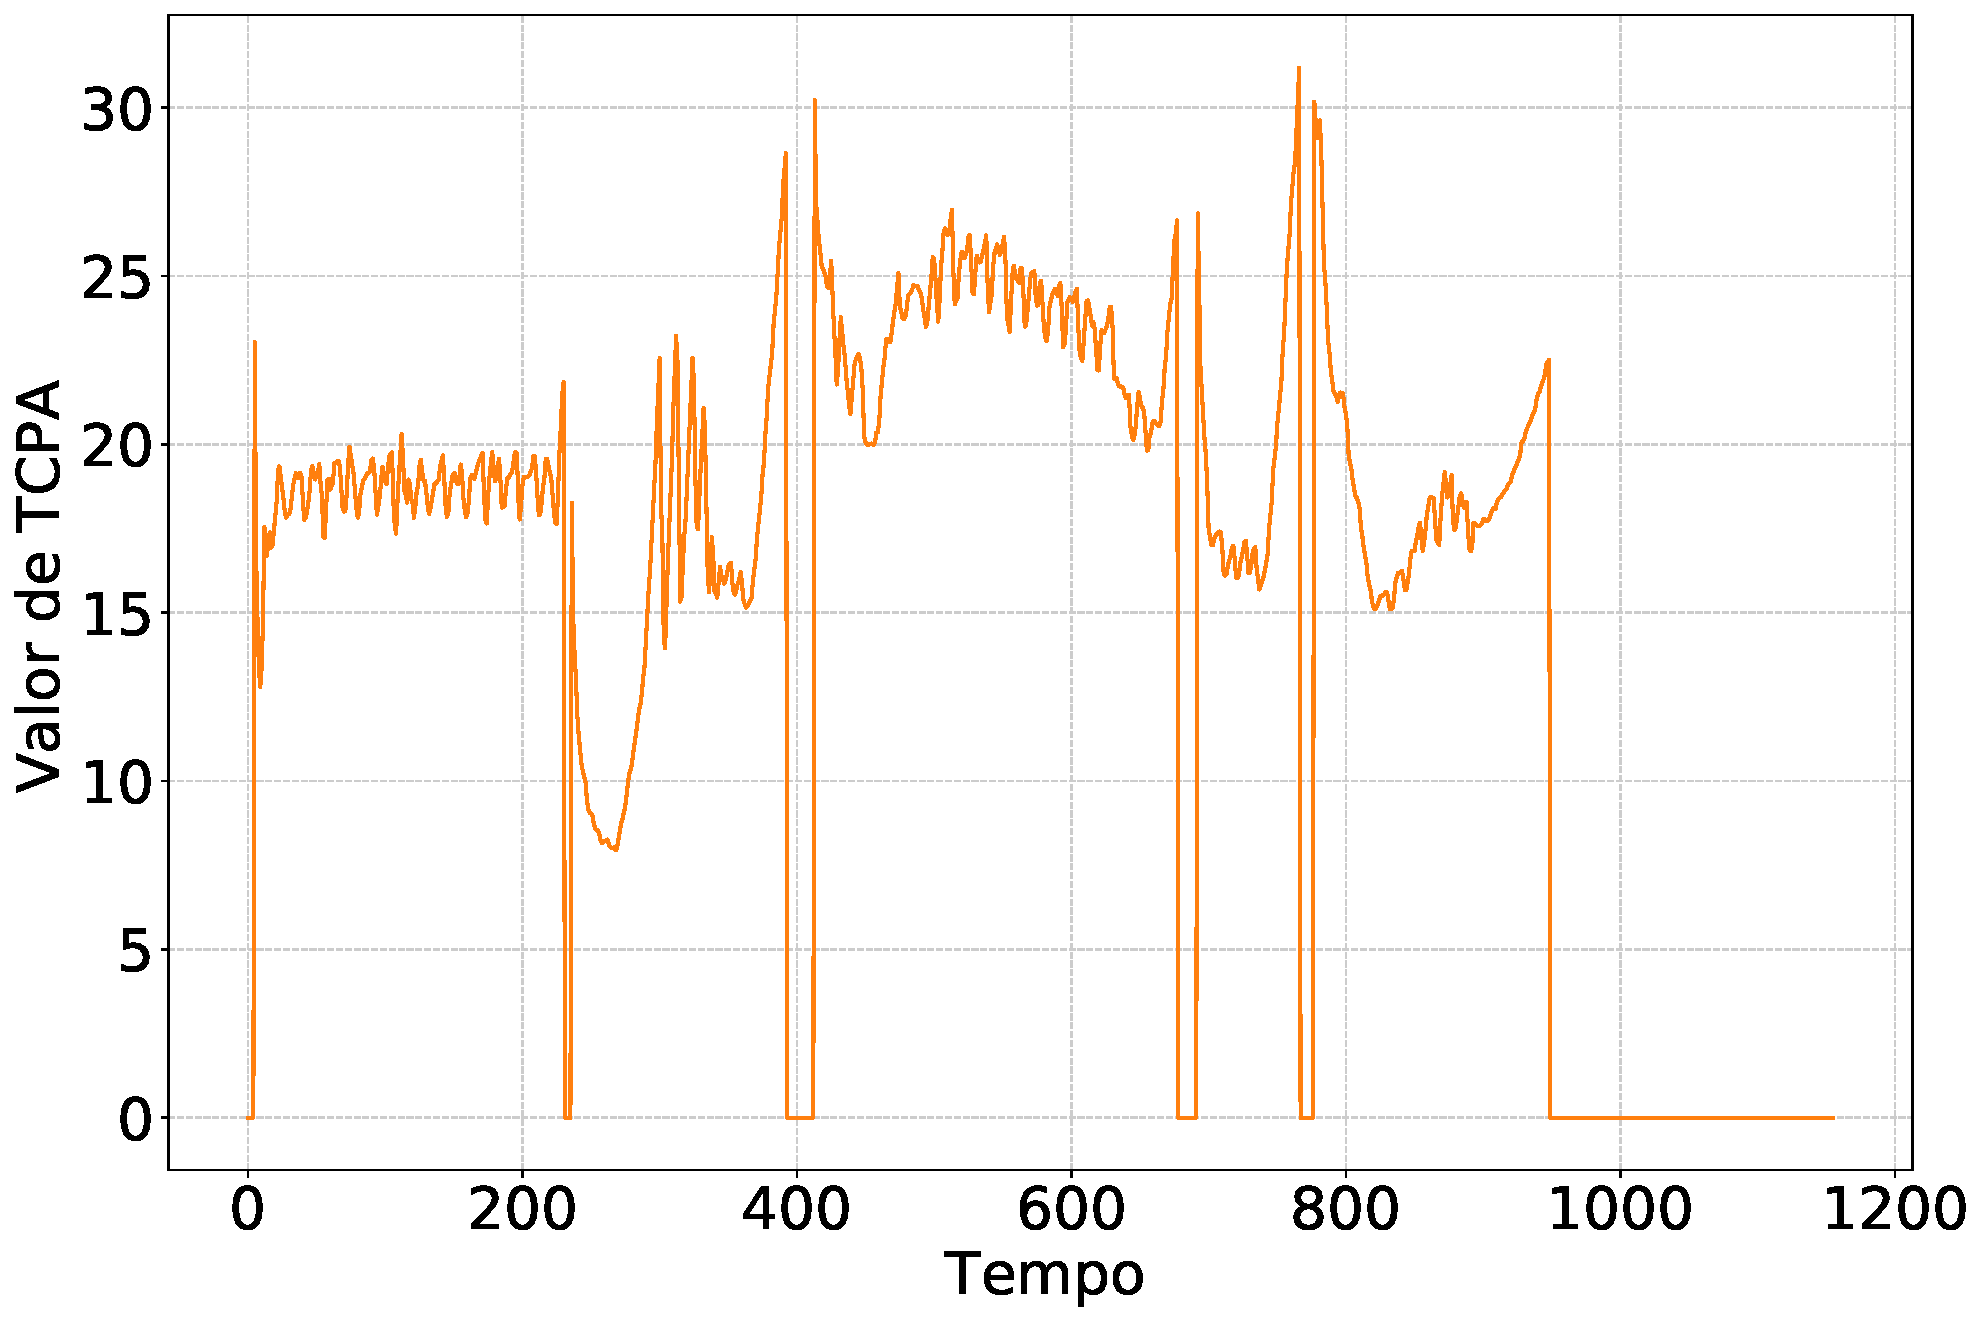
\includegraphics[width=\textwidth]{fig/chap5/crossing_right_stopped_vessel_cpa_tcpa.pdf}
                \caption{TCPA}
                \label{fig:chap5_crossing_right_stopped_vessel_cpa_tcpa}
            \end{subfigure}
            % \begin{subfigure}{0.5\textwidth}
            \begin{subfigure}{1\textwidth}
                \centering
                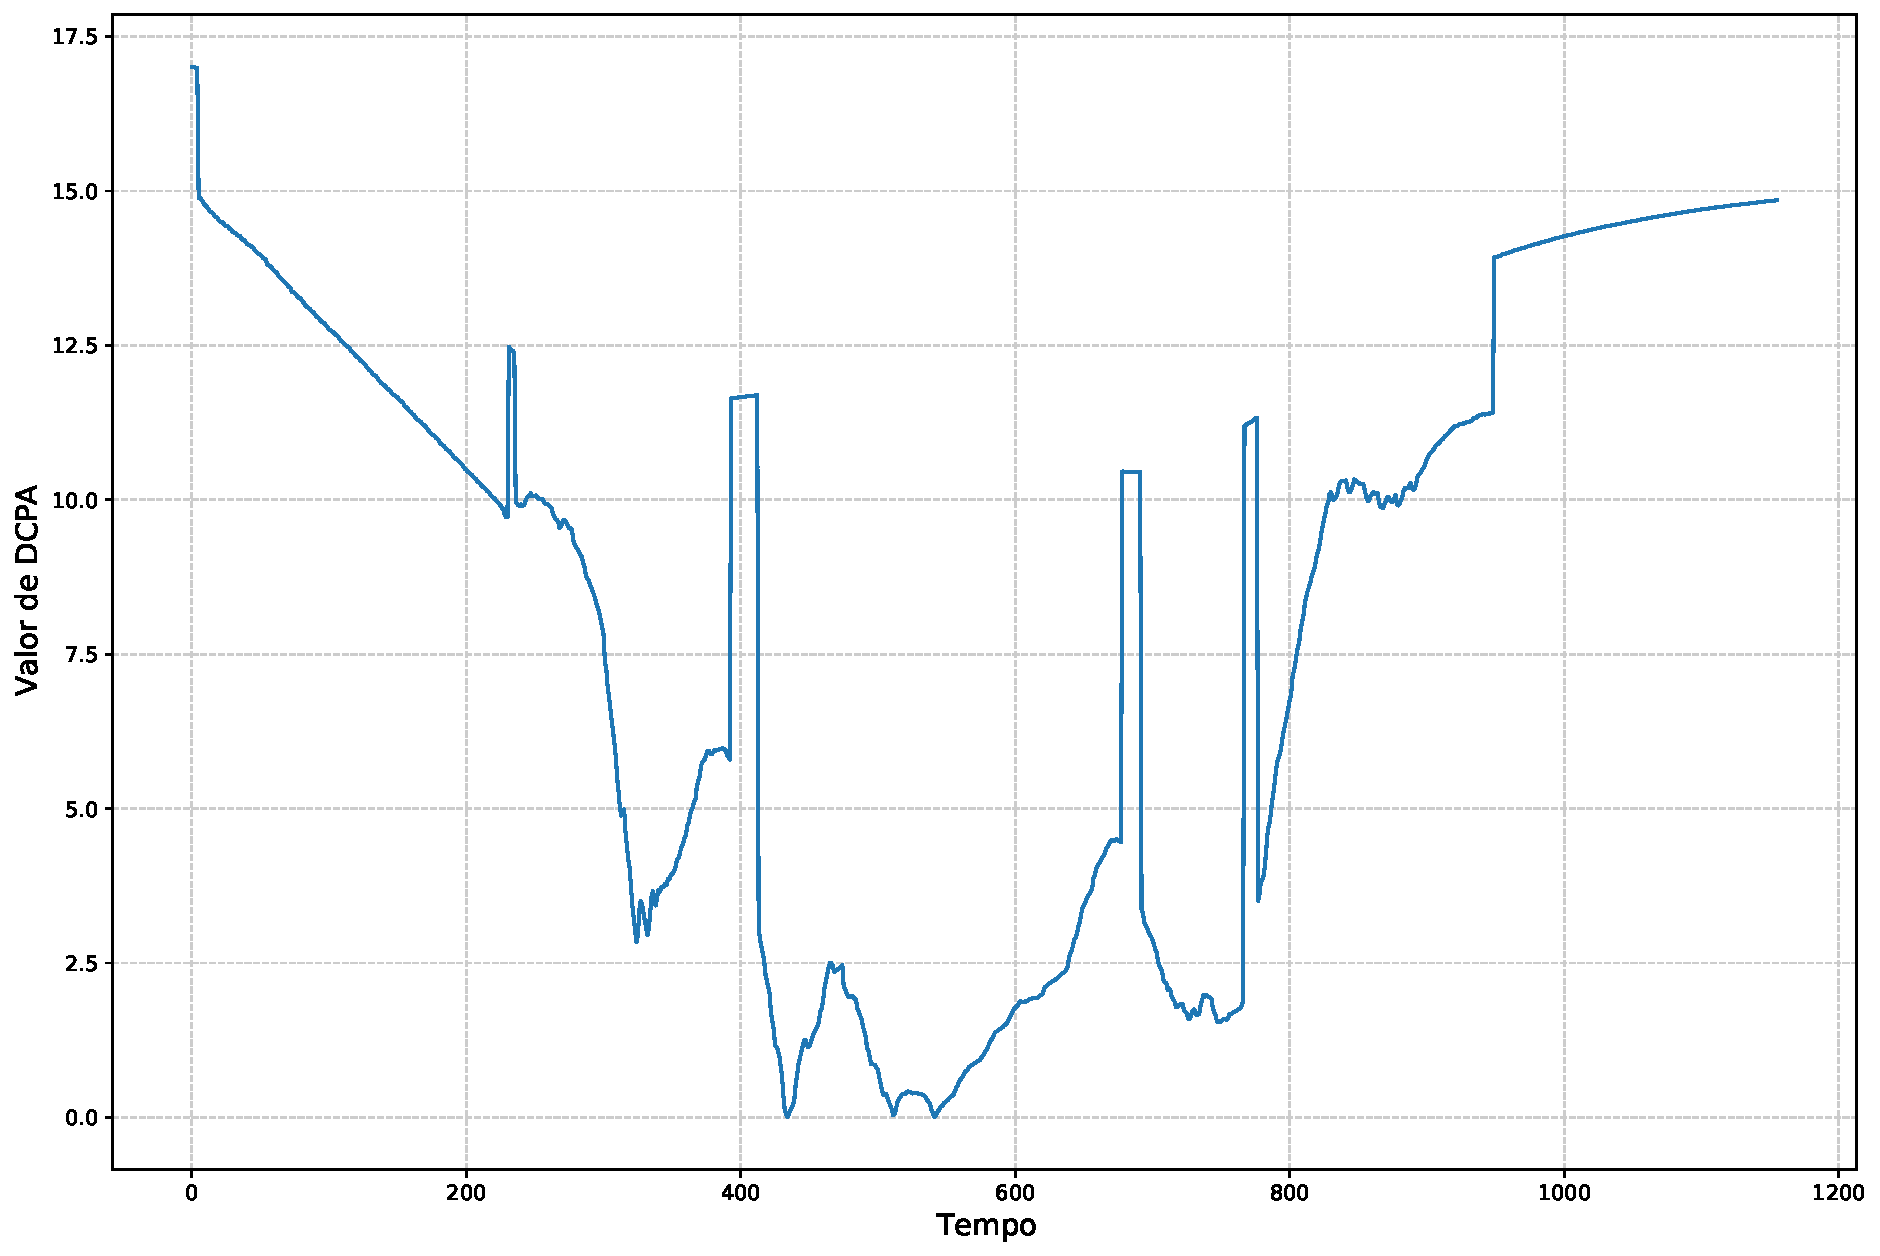
\includegraphics[width=\textwidth]{fig/chap5/crossing_right_stopped_vessel_cpa_dcpa.pdf}
                \caption{DCPA}
                \label{fig:chap5_crossing_right_stopped_vessel_cpa_dcpa}
            \end{subfigure}
            
            \caption{Informações do CPA}
            \label{fig:chap5_crossing_right_stopped_vessel_cpa}
            \end{figure}
            
            \begin{figure}[H]
                \centering
                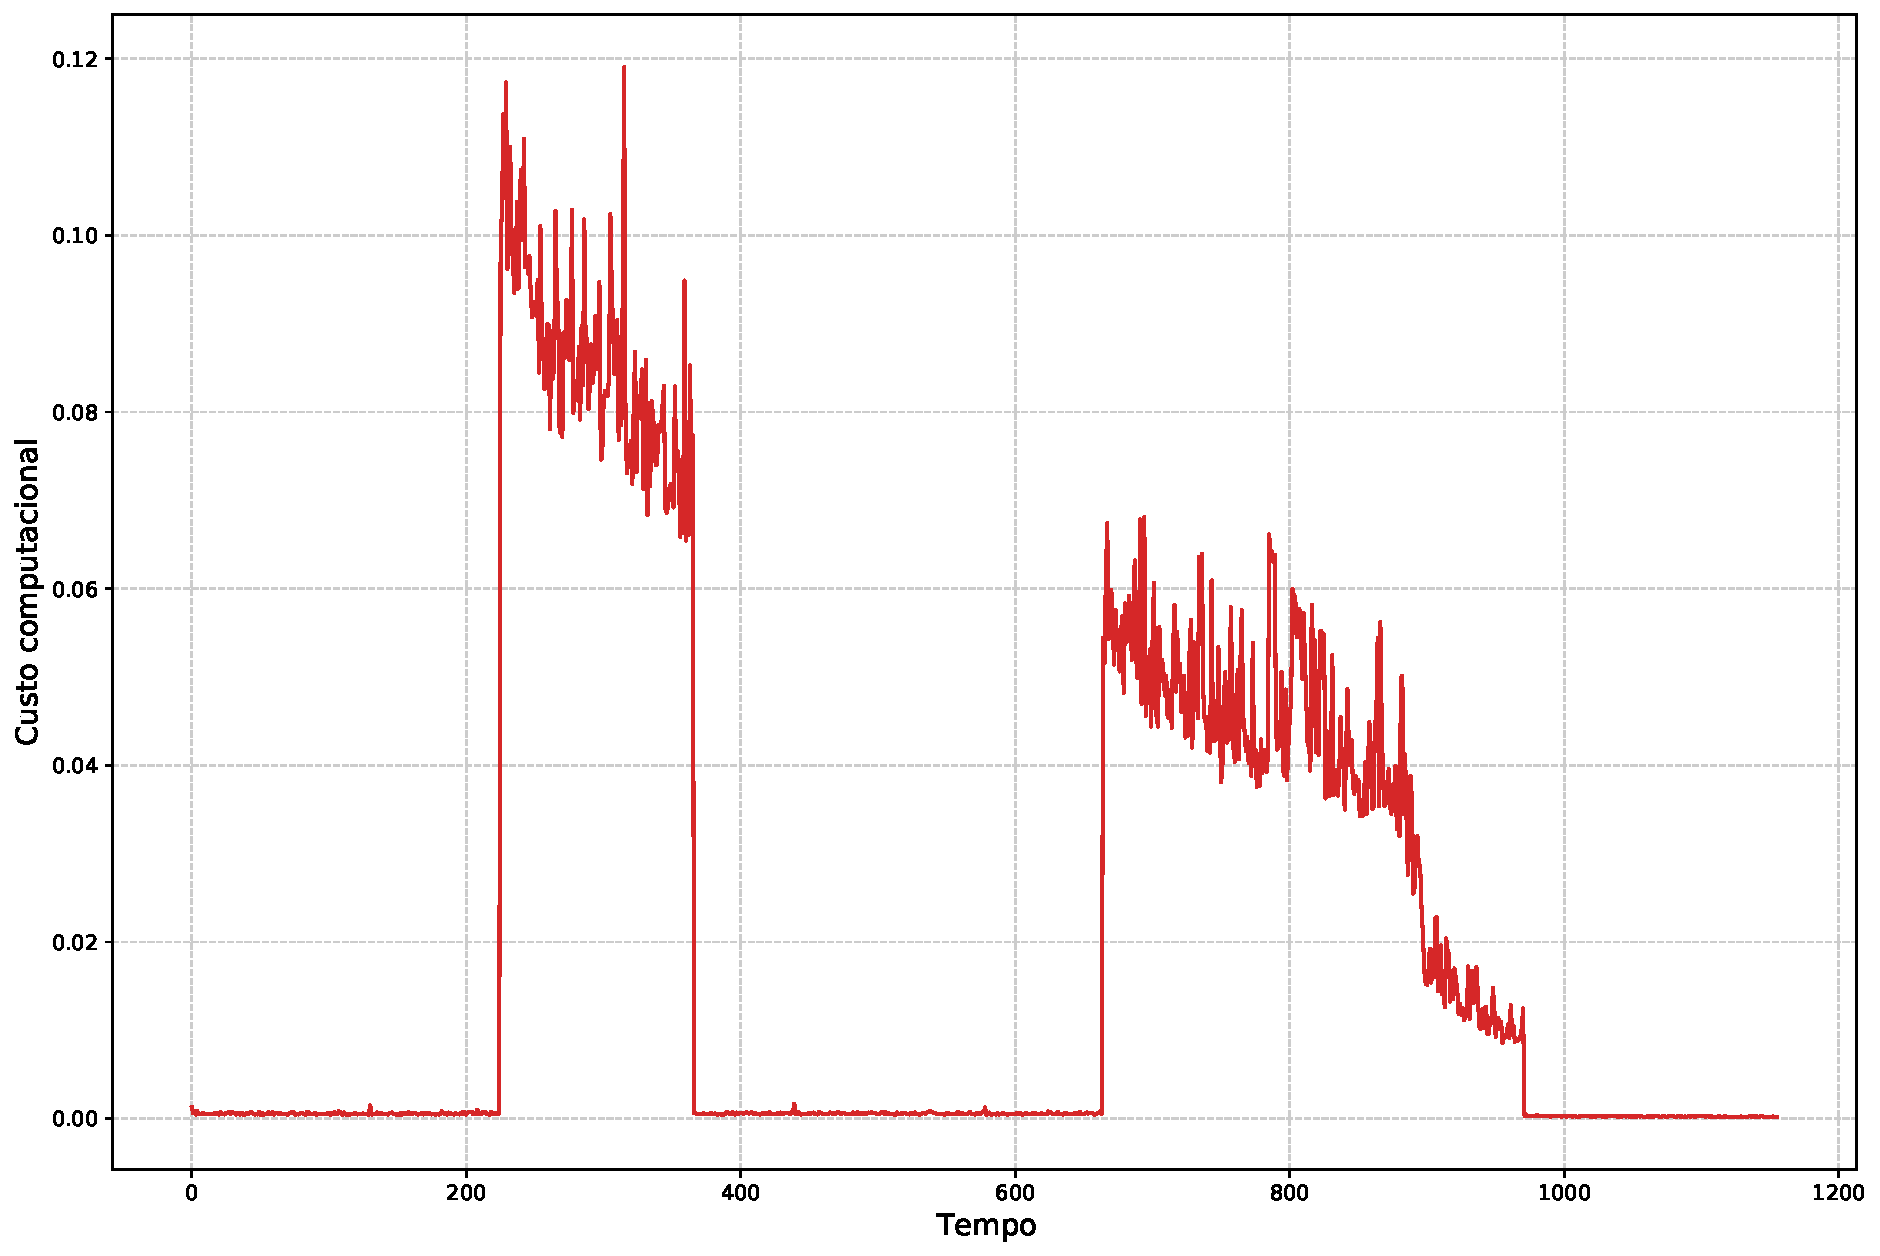
\includegraphics[width=\textwidth]{fig/chap5/crossing_right_stopped_vessel_cpa_computation_time.pdf}
                \caption{Tempo de computação}
                \label{fig:chap5_crossing_right_stopped_vessel_cpa_computation_time}
            \end{figure}
            
    \section{Comparação dos Resultados}
        Como este trabalho se propõe a contribuir com um sistema já existente, faz sentido que comparemos os nossos resultados com os de Jurak~\cite{Jurak2020COLREGS}. A Tabela~\ref{tab:chap5_comparacao_resultados} apresenta as distâncias mínimas obtidas em cada cenário por ambos os trabalhos. Como explicado na Seção~\ref{subchap5_overtake}, para o caso de teste \textit{"Overtake"} obteve-se uma distância menor que o trabalho original pois inicialmente o USV se distanciou de um objeto estático que havia em sua direita, fazendo com que ao ultrapassar a outra embarcação a distância miníma entre elas fosse menor. 
        Já no cenário \textit{"Crossing from Right"}, nossa implementação pode ter impactado para a obtenção de uma distância menor do que o trabalho original, dado que os obstáculos virtuais não são criados exatamente no momento em que o planejador local detecta a outra embarcação como no trabalho original, fazendo com que as embarcações estejam mais próximas no momento em que os obstáculos virtuais são criados. Os casos de teste \textit{"Crossing from Right"} com a outra embarcação parada não foram realizados por Jurak~\cite{Jurak2020COLREGS}, dado que seu sistema 
        não tinha o próposito de avaliar tais situações. Porém ainda assim apresentamos as menores distâncias obtidas como forma de evidenciar a nossa potencial contribuição.
        
        
        \begin{table}[]
            \centering
            \begin{tabular}{|M{5cm}|M{5cm}|M{5cm}|}
                \hline
                Cenário \textbackslash~Autor & Angnes & Jurak \\ [2ex]\hline
                Head On                      & 2,419  & 1,599 \\ [2ex]\hline
                Overtake                     & 2,255  & 3,101 \\ [2ex]\hline
                Crossing Left                & 8,316  & 6,274 \\ [2ex]\hline
                Crossing Right               & 1,866  & 3,264 \\ [2ex]\hline
                Embarcação parada sem CPA    & 1,352  & NA    \\ [2ex]\hline
                Embarcação parada com CPA    & 10,443 & NA    \\ [2ex]\hline
            \end{tabular}
            \caption{Comparação das distâncias mínimas obtidas nos trabalhos}
            \label{tab:chap5_comparacao_resultados}
        \end{table}